\documentclass[letterpaper,12pt]{article}

% --- PAQUETES DE IDIOMA
\usepackage[spanish,mexico]{babel}
\usepackage[utf8]{inputenc}
\usepackage{csquotes}

\usepackage[utf8]{inputenc}
\usepackage[T1]{fontenc}
% --- PAQUETES MATEMÁTICOS --
\usepackage{amsmath}
\usepackage{amssymb}
\usepackage{cancel}
\usepackage{mathrsfs}

% --- PAQUETES GRÁFICOS Y DE DISEÑO ---
\usepackage{graphicx}
\usepackage{float}
\usepackage{subcaption}
\usepackage[table]{xcolor}
\usepackage{longtable}
\usepackage{multirow}
\usepackage{makecell}
\usepackage{array}
\usepackage{caption}
\usepackage{tikz}
\usetikzlibrary{decorations.pathreplacing}
\usetikzlibrary{decorations.pathmorphing}
\usepackage{circuitikz}
\usetikzlibrary{shapes.geometric, shapes.multipart, shapes.symbols, positioning, arrows.meta, calc, shadows, decorations.pathreplacing,babel}

% --- LISTAS ---
\usepackage{enumitem}

% --- PAQUETES DE CÓDIGO ---
\usepackage{listings}
% Configuración del estilo de listings
\definecolor{codebg}{rgb}{0.95,0.95,0.95}   
\definecolor{keyword}{rgb}{0.0,0.2,0.6}     
\definecolor{comment}{rgb}{0.25,0.5,0.35}   
\definecolor{string}{rgb}{0.6,0.0,0.0}      
\definecolor{number}{rgb}{0.5,0.0,0.5}      
\definecolor{codegray}{rgb}{0.5,0.5,0.5}
\definecolor{codepurple}{rgb}{0.58,0,0.82}
\definecolor{backcolour}{rgb}{0.95,0.95,0.95}


% Colores para la Tabla 10-2
\definecolor{headerBlueA}{RGB}{91, 155, 213}   % Azul medio para el encabezado
\definecolor{rowBlueA}{RGB}{233, 242, 250}    % Azul muy claro para la fila
\definecolor{borderBlueA}{RGB}{156, 194, 229} % Azul claro para los bordes

% Colores para la Tabla 10-1
\definecolor{headerBlueB}{RGB}{68, 114, 196}  % Azul oscuro para el encabezado
\definecolor{rowBlueB}{RGB}{217, 225, 242}    % Azul claro para filas intercaladas
\definecolor{borderBlueB}{RGB}{143, 170, 220} % Azul medio para los bordes

% Colores para la Tabla 8-2 (Amarillo/Oro)
\definecolor{hdryellow}{RGB}{255, 192, 0}
\definecolor{row1yellow}{RGB}{255, 242, 204}
\definecolor{row2yellow}{RGB}{255, 249, 227}

% Definición de los colores utilizados en las tablas
\definecolor{headerbg}{HTML}{5B84C4} % Azul oscuro para el encabezado principal
\definecolor{subheaderbg}{HTML}{B4C6E7} % Azul intermedio para sub-encabezados
\definecolor{rowbg}{HTML}{E9EDF4} % Azul claro para filas intercaladas

% Definición de colores exactos para las tablas y semáforo
\definecolor{SemGreen}{RGB}{0, 176, 80}
\definecolor{SemYellow}{RGB}{255, 255, 0}
\definecolor{SemRed}{RGB}{255, 0, 0}

\definecolor{TabOrangeHead}{RGB}{237, 125, 49}
\definecolor{TabOrangeBody}{RGB}{252, 228, 214}

\definecolor{TabGreyHead}{RGB}{165, 165, 165}
\definecolor{TabGreyBody}{RGB}{237, 237, 237}

\definecolor{TabBlueHead}{RGB}{68, 114, 196}
\definecolor{TabBlueBody}{RGB}{217, 225, 242}

\definecolor{keywords}{RGB}{128,0,128}    % Morado para palabras clave
\definecolor{numbers}{RGB}{205,92,92}     % Naranja/Rojo para números
\definecolor{strings}{RGB}{34,139,34}     % Verde para texto
\definecolor{comments}{RGB}{169,169,169}  % Gris para comentarios
\definecolor{background}{RGB}{252,252,252}% Fondo muy claro

\lstset{
    language=Python,
    backgroundcolor=\color{background},
    basicstyle=\ttfamily\normalsize,
    keywordstyle=\color{keywords}\bfseries,
    stringstyle=\color{strings},
    commentstyle=\color{comments}\itshape,
    numberstyle=\color{numbers},
    % Añadir palabras de MicroPython a las keywords
    morekeywords={Pin, I2C, freq, readfrom, from_bytes, hex, range, sleep, scan, port, pin, putstr, clear, move_to, show, text, round, sleep_ms, utime, True, False},
    % Colorear los números
    literate=
        {0}{{{\color{numbers}0}}}1
        {1}{{{\color{numbers}1}}}1
        {2}{{{\color{numbers}2}}}1
        {3}{{{\color{numbers}3}}}1
        {4}{{{\color{numbers}4}}}1
        {5}{{{\color{numbers}5}}}1
        {6}{{{\color{numbers}6}}}1
        {7}{{{\color{numbers}7}}}1
        {8}{{{\color{numbers}8}}}1
        {9}{{{\color{numbers}9}}}1
        {0x39}{{{\color{numbers}0x39}}}4
        {0x3F}{{{\color{numbers}0x3F}}}4
        {0x3E}{{{\color{numbers}0x3E}}}4
        {0x27}{{{\color{numbers}0x27}}}4
        {0x48}{{{\color{numbers}0x48}}}4,
    showstringspaces=false,
    breaklines=true,
    frame=none,
    numbers=none,
    tabsize=4,
    belowcaptionskip=1em,
    abovecaptionskip=1em
}

\lstset{
  backgroundcolor=\color{backcolour},
  basicstyle=\ttfamily\small,
    inputencoding=utf8,
  keywordstyle=\color{blue}\bfseries,
  stringstyle=\color{codepurple},
  commentstyle=\color{codegray}\itshape,
  numbers=left,
  numberstyle=\tiny\color{codegray},
  frame=single,
  rulecolor=\color{black},
  breaklines=true,
  tabsize=4,
  showstringspaces=false,
  extendedchars=true,
  literate={á}{{\'a}}1
           {é}{{\'e}}1
           {í}{{\'i}}1
           {ó}{{\'o}}1
           {ú}{{\'u}}1
           {Á}{{\'A}}1
           {É}{{\'E}}1
           {Í}{{\'I}}1
           {Ó}{{\'O}}1
           {Ú}{{\'U}}1
           {ñ}{{\~n}}1
           {Ñ}{{\~N}}1
           {¿}{{\textquestiondown}}1
           {¡}{{\textexclamdown}}1
           {°}{{\textdegree}}1
           {ø}{{\o}}1
}

% Definición del lenguaje Python para listings
\lstdefinelanguage[LAB]{Python}{
    morekeywords={False, None, True, and, as, assert, async, await, break,
                                class, continue, def, del, elif, else, except, finally,
                                for, from, global, if, import, in, is, lambda, nonlocal,
                                not, or, pass, raise, return, try, while, with, yield,
                                machine, Pin, PWM, ADC, Timer, sleep_ms, sleep_us},
    morecomment=[l]{\#},
    morestring=[b]",
    morestring=[b]',
    sensitive=true
}

% --- ESTILOS PARA DIAGRAMAS DE FLUJO (TIKZ) ---
\tikzset{
  startstop/.style={rectangle, rounded corners, minimum width=3cm, minimum height=1cm,text centered, draw=black, fill=red!30},
  process/.style={rectangle, minimum width=3cm, minimum height=1cm, text centered, draw=black, fill=orange!30},
  decision/.style={diamond, aspect=2, minimum width=3cm, minimum height=1cm, text centered, draw=black, fill=green!30},
  io/.style={trapezium, trapezium left angle=70, trapezium right angle=110, minimum width=3cm, minimum height=1cm, text centered, draw=black, fill=blue!30},
  arrow/.style={thick,->,>=stealth}
}

% Definimos el color dorado/naranja para el cuadro de texto
\definecolor{goldbox}{RGB}{218, 140, 15}

% Macro para dibujar la Raspberry Pi Pico y sus nodos
\newcommand{\picoboard}{
    \draw[thick] (0,0.5) rectangle (4,-9.5);
    \node[align=center, font=\small\sffamily] at (2, -1.5) {Raspberry PI\\[0.1cm]Pico};

    % Pines Superiores
    \draw[red, thick] (0.8, 0.5) -- (0.8, 0.8) coordinate (P41); \node[above, font=\tiny\sffamily, inner sep=1pt] at (P41) {41};
    \draw[red, thick] (2.0, 0.5) -- (2.0, 0.8) coordinate (P42); \node[above, font=\tiny\sffamily, inner sep=1pt] at (P42) {42};
    \draw[red, thick] (3.2, 0.5) -- (3.2, 0.8) coordinate (P43); \node[above, font=\tiny\sffamily, inner sep=1pt] at (P43) {43};
    \node[below, font=\tiny\sffamily] at (0.8, 0.5) {SW CLK};
    \node[below, font=\tiny\sffamily] at (2.0, 0.5) {SW GND};
    \node[below, font=\tiny\sffamily] at (3.2, 0.5) {SW DIO};

    % GND Inferior
    \draw[red, thick] (2, -9.5) -- (2, -10.2) coordinate (PGND);
    \node[above, font=\tiny\sffamily] at (2, -9.5) {GND};
    \node[below, font=\tiny\sffamily] at (2, -10.2) {3,8,13,18 \quad 23,28,38};

    % Pines del lado Izquierdo
    \foreach \i/\pin/\num in {
        1/GP0/1, 2/GP1/2, 
        4/GP2/4, 5/GP3/5, 6/GP4/6, 7/GP5/7, 
        9/GP6/9, 10/GP7/10, 11/GP8/11, 12/GP9/12, 
        14/GP10/14, 15/GP11/15, 16/GP12/16, 17/GP13/17, 
        19/GP14/19, 20/GP15/20
    } {
        \draw[red, thick] (0, -\i*0.45) -- (-0.4, -\i*0.45) coordinate (P\num);
        \node[right, font=\tiny\sffamily] at (0, -\i*0.45) {\pin};
        \node[above left, font=\tiny\sffamily, inner sep=1pt] at (P\num) {\num};
    }

    % Pines del lado Derecho
    \foreach \i/\pin/\num in {
        1/VBUS/40, 2/VSS/39, 
        4/3V3\_EN/37, 5/3V3/36, 6/ADC\_VREF/35, 7/GP28\_A2/34, 8/AGND/33, 
        9/GP27\_A1/32, 10/GP26\_A0/31, 11/RUN/30, 12/GP22/29, 
        14/GP21/27, 15/GP20/26, 16/GP19/25, 17/GP18/24, 
        19/GP17/22, 20/GP16/21
    } {
        \draw[red, thick] (4, -\i*0.45) -- (4.4, -\i*0.45) coordinate (P\num);
        \node[left, font=\tiny\sffamily] at (4, -\i*0.45) {\pin};
        \node[above right, font=\tiny\sffamily, inner sep=1pt] at (P\num) {\num};
    }
}



\definecolor{azulresultado}{HTML}{0072C6}
\definecolor{rojoacarreo}{HTML}{FF0000}

% Colores para la tabla
\definecolor{headblue}{HTML}{4F81BD}
\definecolor{subheadblue}{HTML}{B8CCE4}
\definecolor{datablockblue}{HTML}{DCE6F1}
% Definición de los colores extraídos de la imagen
\definecolor{HeaderBlue}{RGB}{68, 114, 196}  % Azul fuerte del encabezado
\definecolor{RowBlue}{RGB}{217, 225, 242}    % Azul claro de la primera fila
\definecolor{BorderBlue}{RGB}{143, 172, 223} % Azul medio para los bordes

% --- RUTAS DE IMÁGENES ---
\graphicspath{{img/}{portada_img/}}

\definecolor{armblue}{RGB}{0, 113, 188}

% --- CONFIGURACIÓN DE PÁGINA (GEOMETRÍA) ---
\usepackage[
    left=25mm, 
    right=25mm,
    top=35mm,
    bottom=30mm,
    headheight=77pt, 
    papersize={21.59cm,27.94cm}
]{geometry}

% --- FORMATO DE TEXTO ---
\renewcommand{\baselinestretch}{1.25} 
\usepackage{parskip} 
\usepackage{lipsum}  

% --- VARIABLES GLOBALES ---
\newcommand{\materia}{}

% --- ENCABEZADOS Y PIES DE PÁGINA ---
\usepackage{fancyhdr}
\pagestyle{fancy}
\fancyhf{} 
\fancyhead[L]{
\includegraphics[height=1.5cm]{portada_img/der.png}}
\fancyhead[R]{
\includegraphics[height=1.5cm]{portada_img/izq.png}}
\fancyfoot[C]{\thepage} 
\renewcommand{\headrulewidth}{0.4pt} 
\renewcommand{\footrulewidth}{0pt}  

% --- BIBLIOGRAFÍA ---
\usepackage[backend=biber, style=numeric, sorting=none, url=true]{biblatex}
\addbibresource{referencias.bib}

% --- HIPERVÍNCULOS ---
\usepackage{hyperref}
\hypersetup{
    colorlinks=true,
    linkcolor=blue,
    citecolor=blue,
    filecolor=magenta,
    urlcolor=cyan
}

\begin{document}
    \input{portada.tex}

    \newpage
    \setcounter{page}{1}

    \section{Objetivo:}

    Aprender la teoría y aplicación del protocolo I2C, controlar módulos de diversos tipos con comunicación I2C.

    \section*{Actividad 1}

\noindent Escribir el siguiente código, comentar; reportar que hace.

\begin{lstlisting}[basicstyle=\ttfamily\footnotesize, caption={Figura 10-9. Código de prueba; actividad 1}]
from machine import Pin, I2C

sda = Pin(8)
scl = Pin(9)
i2c = I2C(0, scl=scl, sda=sda)

devices = i2c.scan()
if devices:
    for d in devices:
        print(hex(d))
\end{lstlisting}

\section*{Propuesta de solución}

El programa proporcionado implementa un escaneo del bus I2C para detectar todos los dispositivos conectados a la Raspberry Pi Pico. Se configuran los pines GPIO 8 como SDA (\textit{Serial Data Line}) y GPIO 9 como SCL (\textit{Serial Clock Line}), que corresponden al bus I2C numero 0. Mediante el metodo \texttt{scan()} se realiza un barrido por todas las direcciones I2C posibles (de 0x08 a 0x77). Cada direccion donde un dispositivo responde confirmando su presencia se almacena en la lista \texttt{devices}. Finalmente, si se encontraron dispositivos, se imprimen sus direcciones en formato hexadecimal; de lo contrario, se informa que no se detecto ninguno.

% Diagrama de flujo
\begin{center}
    \scalebox{0.85}{
    \begin{tikzpicture}[node distance=1.05cm, every node/.style={font=\scriptsize}]
        \node (start1) [startstop, text width=2.6cm] {Inicio};
        \node (init1) [process, below=of start1, text width=7.5cm] {Importar \texttt{Pin} y \texttt{I2C} desde \texttt{machine}.};
        \node (config1) [process, below=of init1, text width=7.5cm] {Configurar SDA en GPIO 8 y SCL en GPIO 9. Inicializar bus I2C(0).};
        \node (scan1) [process, below=of config1, text width=5.8cm] {Ejecutar \texttt{i2c.scan()} para detectar dispositivos.};
        \node (decision1) [decision, below=of scan1, text width=4.0cm, aspect=2.2] {¿\texttt{devices} tiene elementos?};
        
        % Bloque para "Si" (va abajo)
        \node (print1) [process, below=of decision1, text width=6.5cm] {Recorrer \texttt{devices} e imprimir direcciones en hexadecimal.};
        
        % Bloque para "No" (va a la derecha)
        \node (nofound1) [process, right=2.5cm of decision1, text width=5.5cm] {Imprimir "No se encontraron dispositivos".};
        
        \node (end1) [startstop, below=of print1, text width=2.0cm] {Fin};
        
        \draw [arrow] (start1) -- (init1);
        \draw [arrow] (init1) -- (config1);
        \draw [arrow] (config1) -- (scan1);
        \draw [arrow] (scan1) -- (decision1);
        
        \draw [arrow] (decision1.south) -- node[right, font=\scriptsize] {Si} (print1.north);
        
        % Flecha "No" - sale por la derecha hacia nofound1
        \draw [arrow] (decision1.east) -- node[above, font=\scriptsize] {No} (nofound1.west);
        
        % Flecha desde print1 hacia Fin
        \draw [arrow] (print1) -- (end1);
        
        % Flecha desde nofound1 hacia Fin (baja y luego entra por la derecha de Fin)
        \draw [arrow] (nofound1.south) |- (end1.east);
        
    \end{tikzpicture}
    }
\end{center}

\section*{Desarrollo}

\lstinputlisting[language={[LAB]Python}, caption=Código comentado de la Actividad 1, basicstyle=\ttfamily\scriptsize]{Code/Act1.py}

\begin{figure}[H]
    \centering
    
\includegraphics[width=0.75\textwidth]{img/Actividad1/Act1_1.jpg}
    \caption{Salida en consola mostrando los dispositivos I2C detectados a la pico.}
\end{figure}

\subsection*{Análisis de resultados}

El programa logra escanear exitosamente el bus I2C y detectar cinco dispositivos conectados a la Raspberry Pi Pico, cuyas direcciones hexadecimales son 0x21, 0x27, 0x38, 0x3c y 0x68. La direccion 0x3c corresponde tipicamente a un display OLED, la 0x68 a un MPU6050 (acelerometro/giroscopio), y las restantes podrian ser expansores de puertos o modulos RTC. El uso del metodo \texttt{scan()} automatiza completamente la deteccion sin necesidad de conocer previamente las direcciones de los dispositivos. El bus I2C configurado en los pines GPIO 8 y 9 funciono correctamente, y la impresion en formato \texttt{hex(d)} facilita la identificacion de cada periferico para su posterior uso en programas mas complejos y el \texttt{if devices} maneja adecuadamente el caso de que no haya dispositivos conectados.


    \newpage
    \section*{Actividad 2}

\noindent Escribir, comentar e indicar el funcionamiento del siguiente c\'odigo, ser\'a empleada la comunicaci\'on serie I2C usando el circuito PCF8574; estudiar la librer\'ia empleada.

\begin{center}
\resizebox{\linewidth}{!}{
\begin{tikzpicture}[>=latex]

% Macro para el circuito integrado PCF8574
\newcommand{\pcfboard}{
    \draw[thick, fill=white] (-1.5, 1.0) rectangle (1.5, -2.6);
    \node[align=center, font=\small\sffamily] at (0, -0.8) {PCF8574};
    
    % Pines lado Izquierdo
    \foreach \i/\pin/\num in {0/A0/1, 1/A1/2, 2/A2/3, 3/P0/4, 4/P1/5, 5/P2/6, 6/P3/7, 7/GND/8} {
        \draw[red, thick] (-1.5, 0.6-\i*0.4) -- (-1.9, 0.6-\i*0.4) coordinate (PCF\num);
        \node[right, font=\tiny\sffamily] at (-1.5, 0.6-\i*0.4) {\pin};
        \node[above, font=\tiny\sffamily, inner sep=1pt] at (-1.7, 0.6-\i*0.4) {\num};
    }
    
    % Pines lado Derecho
    \foreach \i/\pin/\num in {7/P4/9, 6/P5/10, 5/P6/11, 4/P7/12, 3/INT/13, 2/SCL/14, 1/SDA/15, 0/VCC/16} {
        \draw[red, thick] (1.5, 0.6-\i*0.4) -- (1.9, 0.6-\i*0.4) coordinate (PCF\num);
        \node[left, font=\tiny\sffamily] at (1.5, 0.6-\i*0.4) {\pin};
        \node[above, font=\tiny\sffamily, inner sep=1pt] at (1.7, 0.6-\i*0.4) {\num};
    }
}

% -------------------------------------------------------------
% DIBUJO DE COMPONENTES Y RUTEOS
% -------------------------------------------------------------

% 1. Pico desplazada hacia arriba
\begin{scope}[xshift=8cm, yshift=5.15cm]
    \picoboard
\end{scope}

% 2. PCF8574 en el centro
\begin{scope}[xshift=0cm, yshift=0cm]
    \pcfboard
\end{scope}

% 3. Conexiones I2C (PCF a Pico)
\draw[yellow, thick] (PCF15) -- (P11);  % SDA a GP8
\draw[brown, thick] (PCF14) -- (4.0, -0.2) |- (P12); % SCL a GP9

% ================= LADO DERECHO ================= 

% Alimentacion VCC (Pin 16)
\draw[thick] (PCF16) -- ++(0.5,0) |- ++(0, 1.2) node[vcc]{3.3V};

% Boton S4 (Pin 12 / P7) 
\draw[magenta, thick] (PCF12) -| (3.5, 3.0) -- (4.0, 3.0);
\draw (4.0, 3.0) to[nopb, l=S4] (6.0, 3.0) node[ground]{};

% RGB2 - Escalonado hacia ABAJO
\draw[cyan, thick] (PCF11) -| (3.2, -1.5) -- (4.0, -1.5);
\draw (6.0, -1.5) to[leDo, l_=G] (4.0, -1.5);

\draw[green, thick] (PCF10) -| (2.9, -3.0) -- (4.0, -3.0);
\draw (6.0, -3.0) to[leDo, l_=B] (4.0, -3.0);

\draw[blue, thick] (PCF9) -| (2.6, -4.5) -- (4.0, -4.5);
\draw (6.0, -4.5) to[leDo, l_=R] (4.0, -4.5);

% Union de anodos RGB2 
\draw[thick] (6.0, -1.5) -- (6.0, -4.5); 
\draw[thick] (6.0, -3.0) -- (6.8, -3.0) node[vcc]{3.3V};
\node[right, font=\small\sffamily] at (6.3, -4.5) {RGB2};

% ================= LADO IZQUIERDO ================= 

% Alimentacion A0 (Pin 1)
\draw[thick] (PCF1) -- ++(-0.5,0) |- ++(0, 1.2) node[vcc]{3.3V};

% Pines GND (Pines 2, 3 y 8)
\draw[thick] (PCF2) -- ++(-4.0,0) node[ground]{};
\draw[thick] (PCF3) -- ++(-2.4,0) node[ground]{};
\draw[thick] (PCF8) -- ++(-0.35,0) |- ++(0, -0.6) node[ground]{};

% RGB1 - Escalonado hacia ABAJO
\draw[blue, thick] (PCF4) -| (-3.5, -1.0) -- (-4.0, -1.0);
\draw (-6.0, -1.0) to[leDo, l=G] (-4.0, -1.0);

\draw[green, thick] (PCF5) -| (-3.2, -2.5) -- (-4.0, -2.5);
\draw (-6.0, -2.5) to[leDo, l=B] (-4.0, -2.5);

\draw[cyan, thick] (PCF6) -| (-2.9, -4.0) -- (-4.0, -4.0);
\draw (-6.0, -4.0) to[leDo, l=R] (-4.0, -4.0);

% Union de anodos RGB1
\draw[thick] (-6.0, -1.0) -- (-6.0, -4.0); 
\draw[thick] (-6.0, -2.5) -- (-7.0, -2.5) node[vcc]{3.3V};
\node[left, font=\small\sffamily] at (-6.3, -0.5) {RGB1};

% Boton S3 (Pin 7 / P3) 
\draw[orange, thick] (PCF7) -| (-2.6, -5.5) -- (-4.0, -5.5);
\draw (-4.0, -5.5) to[nopb, l_=S3] (-6.0, -5.5) node[ground]{};

\end{tikzpicture}
}
\end{center}

\begin{lstlisting}[basicstyle=\ttfamily\footnotesize,caption={Figura 10-10. C\'odigo de ejemplo; actividad 2}]
import pcf8574
from machine import I2C, Pin
import time

i2c = I2C (0,scl=Pin(9), sda=Pin(8))
pcf = pcf8574.PCF8574(i2c, 0x39)

while True:
    pcf.port = 0x3F
    print(pcf.port)
    time.sleep(0.8)

    pcf.port = 0x3E
    print(pcf.port)
    time.sleep(0.8)
\end{lstlisting}

\section*{Propuesta de solución}

El programa proporcionado implementa un expansor de pines PCF8574 para controlar 8 salidas digitales a través de solo dos líneas del bus I2C (SDA en GPIO 8 y SCL que en GPIO 9) y para ello se utiliza la librería \texttt{pcf8574} simplifica la escritura sobre el puerto paralelo del dispositivo. Se configura el expansor en la dirección hexadecimal 0x39 correspondiente a las conexiones A0, A1 y A2 a nivel alto o bajo. Dentro del ciclo infinito, se asigna el valor \texttt{0x3F} (binario 00111111) al puerto, lo que pone los pines P0 a P5 en nivel alto (1 lógico) y los pines P6 y P7 en bajo (0 lógico), activando los LEDS. Luego de 0.8 segundos, se asigna \texttt{0x3E} (00111110), que pone el pin P0 en bajo mientras mantiene los demás en alto.

\subsection*{Investigación de la librería \texttt{pcf8574}}

La librer\'ia \texttt{pcf8574} para MicroPython proporciona una interfaz para controlar el expansor de pines PCF8574/PCF8574A a trav\'es del bus I2C. Sus principales caracter\'isticas son:

\begin{itemize}
    \item \texttt{PCF8574(i2c, address)}: Constructor que recibe el objeto I2C configurado y la direcci\'on de 7 bits del dispositivo (com\'unmente 0x20 para PCF8574 o 0x38 para PCF8574A, m\'as el valor de los pines A0-A2).
    \item \texttt{port}: Propiedad que permite leer o escribir el estado completo de los 8 pines como un byte. Al escribir, cada bit corresponde a un pin (bit0 = P0, bit1 = P1, ..., bit7 = P7). Al leer, devuelve el estado actual de los pines considerando si est\'an configurados como entrada o salida.
    \item \texttt{pin(pin, value)}: M\'etodo alternativo para controlar un pin individual sin afectar los dem\'as.
    \item La librer\'ia maneja autom\'aticamente la se\~nal de acknowledge del I2C y la configuraci\'on del registro de salida del PCF8574.
\end{itemize}

% Diagrama de flujo corregido Actividad 2
\begin{center}
    \scalebox{0.82}{
    \begin{tikzpicture}[node distance=1.1cm, every node/.style={font=\scriptsize}]
        \node (start2) [startstop, text width=2.6cm] {Inicio};
        \node (init2) [process, below=of start2, text width=8.2cm] {Importar librerías: \texttt{pcf8574}, \texttt{I2C}, \texttt{Pin}, \texttt{time}.};
        \node (config2) [process, below=of init2, text width=7.5cm] {Configurar I2C(0) con SDA=GP8, SCL=GP9. Crear objeto \texttt{pcf} en dirección \texttt{0x21}.};
        \node (loop2) [process, below=of config2, text width=4.2cm] {\texttt{while True}: Iniciar ciclo infinito.};
        
        % Bloques internos del ciclo
        \node (port3f2) [process, below=of loop2, text width=6.5cm] {Asignar \texttt{pcf.port = 0x3F} (111111). Imprimir estado.};
        \node (wait12) [process, below=of port3f2, text width=4.2cm] {Esperar 0.8 segundos.};
        \node (port3e2) [process, below=of wait12, text width=6.5cm] {Asignar \texttt{pcf.port = 0x3E} (111110). Imprimir estado.};
        \node (wait22) [process, below=of port3e2, text width=4.2cm] {Esperar 0.8 segundos.};
        
        % Conexiones lineales
        \draw [arrow] (start2) -- (init2);
        \draw [arrow] (init2) -- (config2);
        \draw [arrow] (config2) -- (loop2);
        \draw [arrow] (loop2) -- (port3f2);
        \draw [arrow] (port3f2) -- (wait12);
        \draw [arrow] (wait12) -- (port3e2);
        \draw [arrow] (port3e2) -- (wait22);
        
        % Flecha de retorno corregida (sale de abajo de wait22 y entra al lateral de port3f2)
        \draw [arrow] (wait22.south) -- ++(0,-0.5) -- ++(-4.0,0) |- (port3f2.west);
        
    \end{tikzpicture}
    }
\end{center}

\section*{Desarrollo}

\lstinputlisting[language={[LAB]Python}, caption=C\'odigo de la Actividad 2, basicstyle=\ttfamily\scriptsize]{Code/Act2.py}

\begin{figure}[H]
    \centering
    
\includegraphics[width=0.5\textwidth, angle=90]{img/Actividad2/Act2_1.jpg}
    \caption{Estado de encendido del led.}
\end{figure}

\begin{figure}[H]
    \centering
    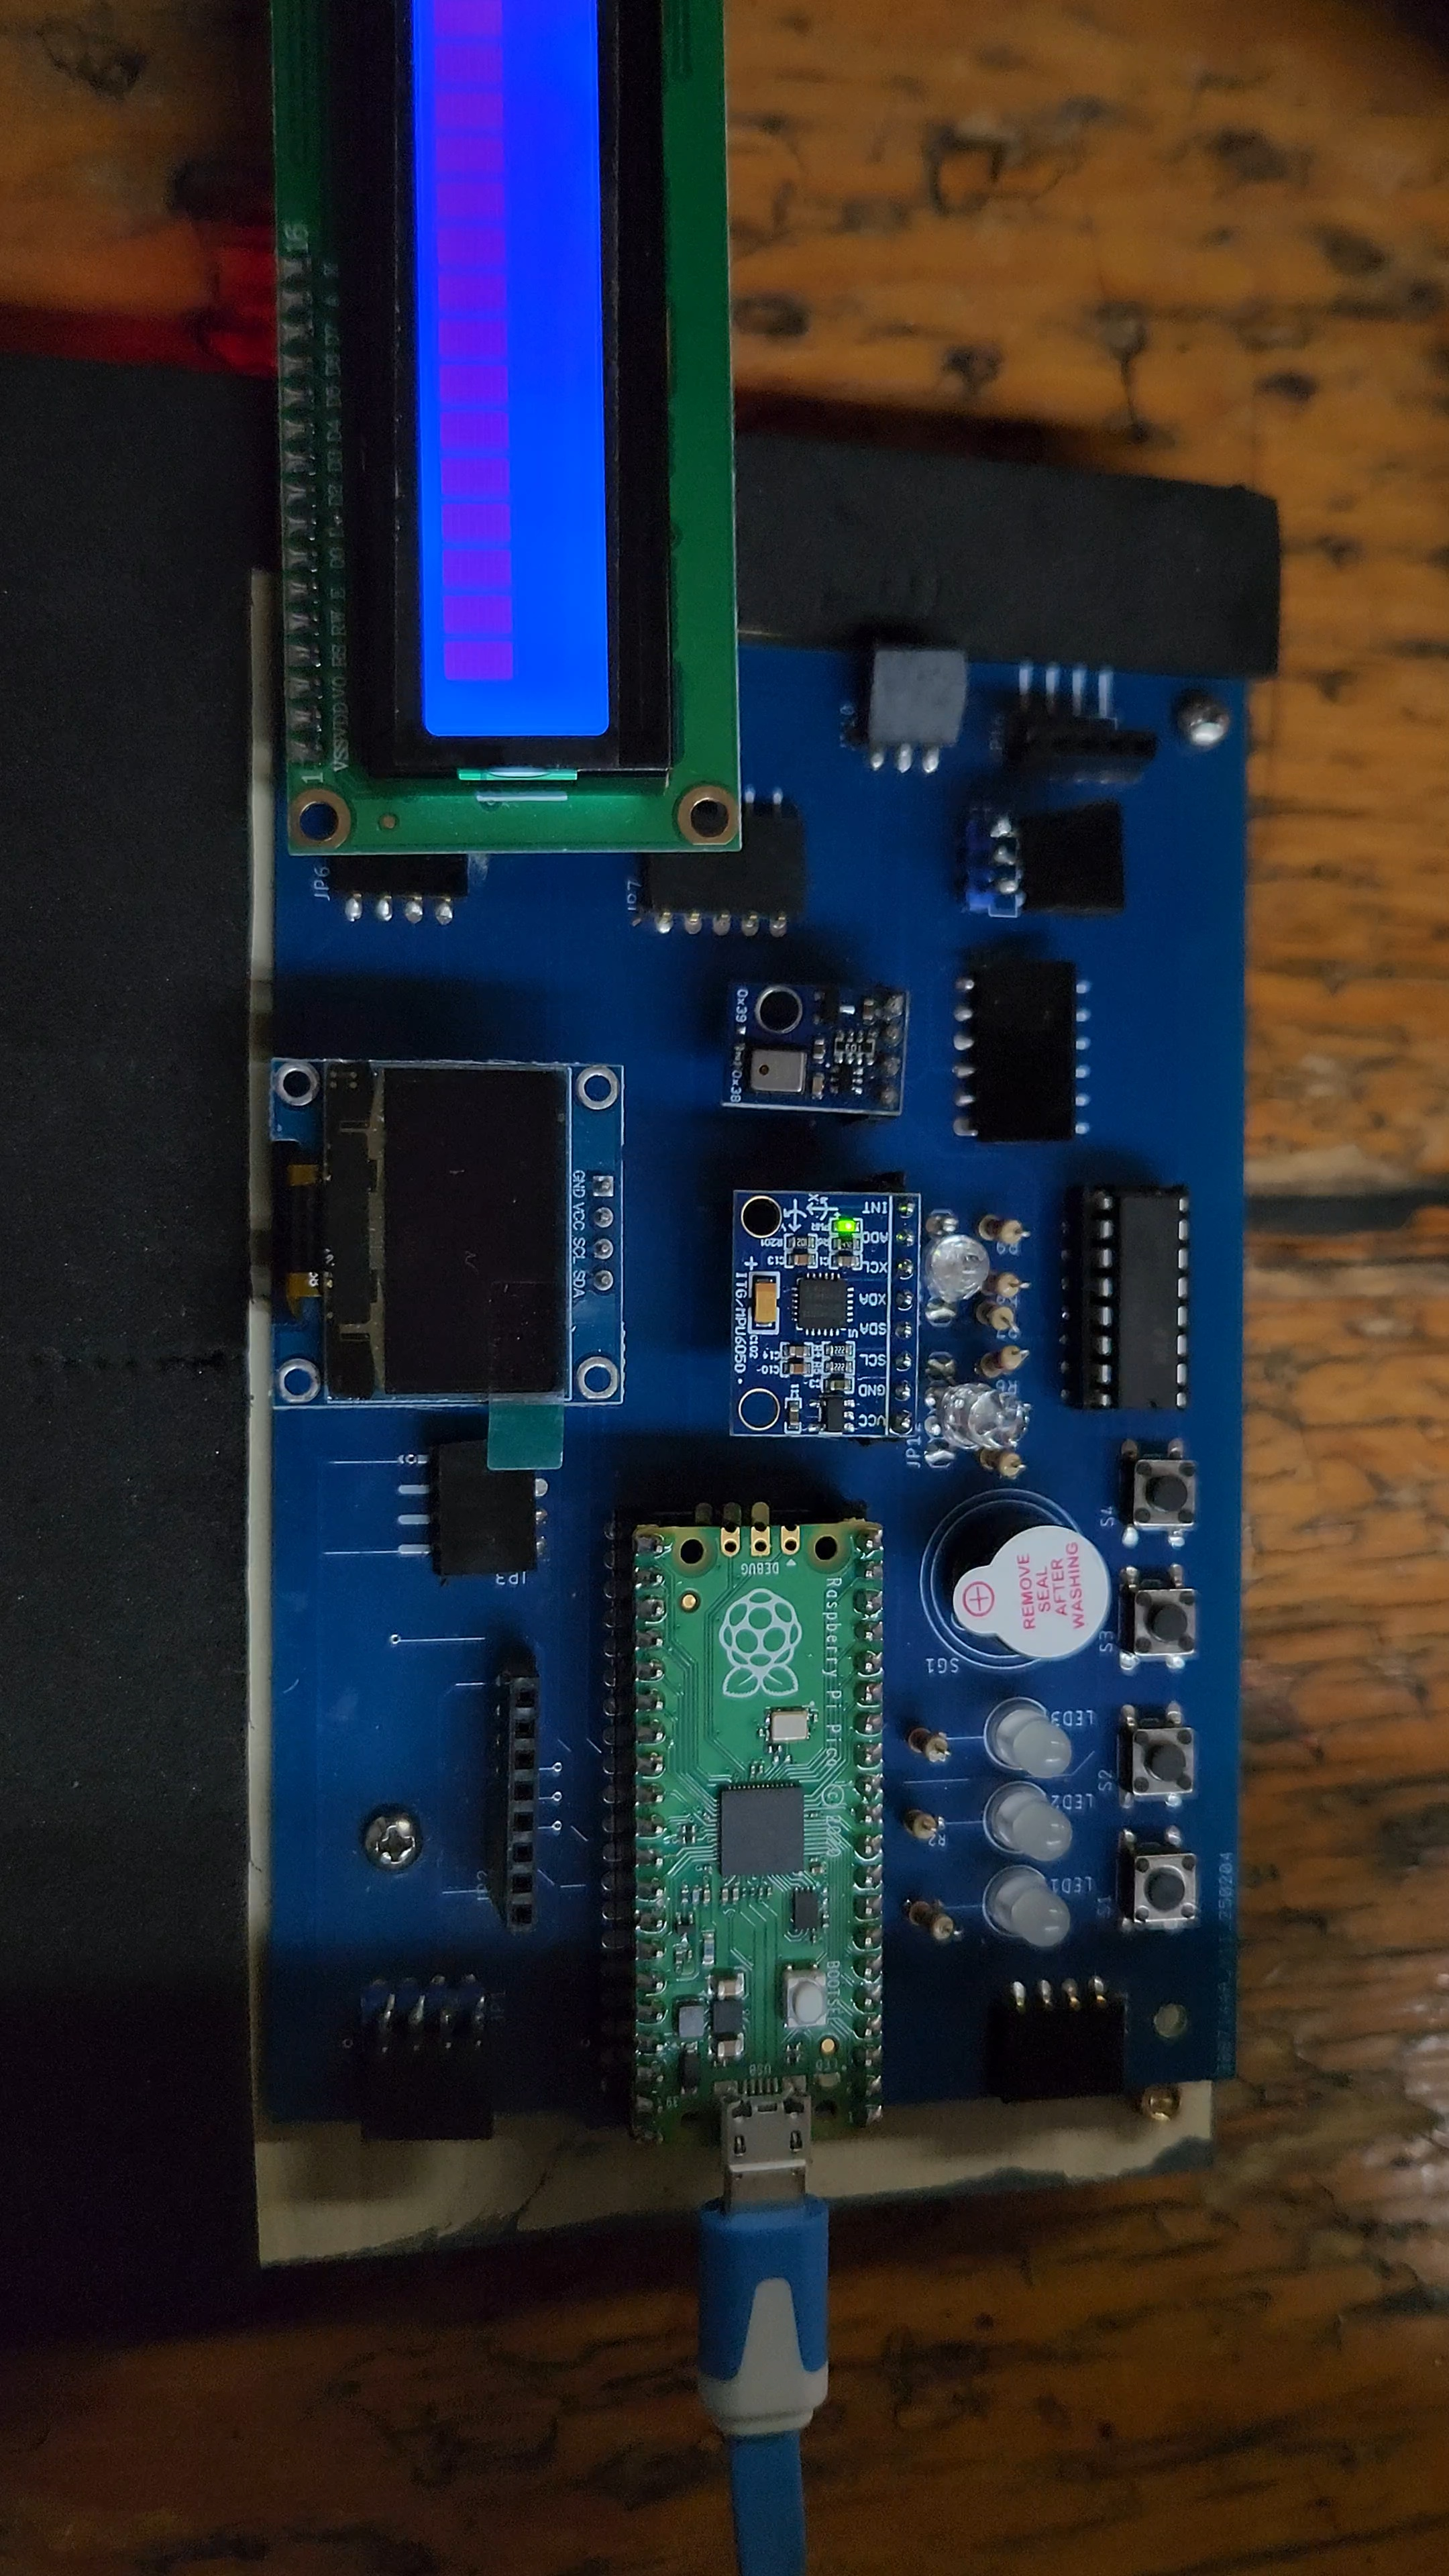
\includegraphics[width=0.5\textwidth, angle=90]{img/Actividad2/Act2_2.jpg}
    \caption{Estado de apagado del led.}
\end{figure}

\subsection*{Análisis de resultados}

El programa logra controlar los 8 pines del PCF8574 mediante la comunicación I2C desde la Raspberry Pi Pico. Al asignar \texttt{0x3F} (00111111), los pines P0 a P5 se ponen en nivel alto, activando los componentes conectados a esas salidas como el LED que se enciende y apaga infiitamente. El uso de la propiedad \texttt{port} simplifica la escritura simultánea de todos los pines sin necesidad de modificar bits individualmente. El retardo de 0.8 segundos entre estados crea un efecto de parpadeo perceptible que permite verificar el cambio de estado. La dirección \texttt{0x39} corresponde a un PCF8574A con A0=1, A1=0, A2=0 (0x38 + 1 = 0x39), confirmando la correcta configuración de los pines de direccionamiento en el hardware y todo esto fue posible gracias a la librería \texttt{pcf8574} que abstrae completamente los detalles del protocolo I2C.


    \newpage
    \section*{Actividad 3}

    \noindent  Utilizando el circuito anterior, generar la secuencia mostrada en la tabla 10-1; considerar comunicación I2C.

        \begin{center}
    \resizebox{\linewidth}{!}{
    \begin{tikzpicture}[>=latex]

    % Macro para el circuito integrado PCF8574
    \newcommand{\pcfboard}{
        \draw[thick, fill=white] (-1.5, 1.0) rectangle (1.5, -2.6);
        \node[align=center, font=\small\sffamily] at (0, -0.8) {PCF8574};
        
        % Pines lado Izquierdo
        \foreach \i/\pin/\num in {0/A0/1, 1/A1/2, 2/A2/3, 3/P0/4, 4/P1/5, 5/P2/6, 6/P3/7, 7/GND/8} {
            \draw[red, thick] (-1.5, 0.6-\i*0.4) -- (-1.9, 0.6-\i*0.4) coordinate (PCF\num);
            \node[right, font=\tiny\sffamily] at (-1.5, 0.6-\i*0.4) {\pin};
            \node[above, font=\tiny\sffamily, inner sep=1pt] at (-1.7, 0.6-\i*0.4) {\num};
        }
        
        % Pines lado Derecho
        \foreach \i/\pin/\num in {7/P4/9, 6/P5/10, 5/P6/11, 4/P7/12, 3/INT/13, 2/SCL/14, 1/SDA/15, 0/VCC/16} {
            \draw[red, thick] (1.5, 0.6-\i*0.4) -- (1.9, 0.6-\i*0.4) coordinate (PCF\num);
            \node[left, font=\tiny\sffamily] at (1.5, 0.6-\i*0.4) {\pin};
            \node[above, font=\tiny\sffamily, inner sep=1pt] at (1.7, 0.6-\i*0.4) {\num};
        }
    }

    % -------------------------------------------------------------
    % DIBUJO DE COMPONENTES Y RUTEOS
    % -------------------------------------------------------------

    % 1. Pico desplazada hacia arriba (Alineación con pines I2C)
    \begin{scope}[xshift=8cm, yshift=5.15cm]
        \picoboard
    \end{scope}

    % 2. PCF8574 en el centro
    \begin{scope}[xshift=0cm, yshift=0cm]
        \pcfboard
    \end{scope}

    % 3. Conexiones I2C (PCF a Pico)
    \draw[yellow, thick] (PCF15) -- (P11);  % SDA a GP8
    \draw[brown, thick] (PCF14) -- (4.0, -0.2) |- (P12); % SCL a GP9

    % ================= LADO DERECHO ================= 

    % Alimentación VCC (Pin 16) - Totalmente aislado para subir a 3.3V
    \draw[thick] (PCF16) -- ++(0.5,0) |- ++(0, 1.2) node[vcc]{3.3V};

    % Botón S4 (Pin 12 / P7) 
    \draw[magenta, thick] (PCF12) -| (3.5, 3.0) -- (4.0, 3.0);
    \draw (4.0, 3.0) to[nopb, l=S4] (6.0, 3.0) node[ground]{};

    % RGB2 - Escalonado hacia ABAJO
    \draw[cyan, thick] (PCF11) -| (3.2, -1.5) -- (4.0, -1.5); % P6 -> G 
    \draw (6.0, -1.5) to[leDo, l_=G] (4.0, -1.5);

    \draw[green, thick] (PCF10) -| (2.9, -3.0) -- (4.0, -3.0); % P5 -> B 
    \draw (6.0, -3.0) to[leDo, l_=B] (4.0, -3.0);

    \draw[blue, thick] (PCF9) -| (2.6, -4.5) -- (4.0, -4.5);  % P4 -> R 
    \draw (6.0, -4.5) to[leDo, l_=R] (4.0, -4.5);

    % Unión de ánodos RGB2 
    \draw[thick] (6.0, -1.5) -- (6.0, -4.5); 
    \draw[thick] (6.0, -3.0) -- (6.8, -3.0) node[vcc]{3.3V};
    \node[right, font=\small\sffamily] at (6.3, -4.5) {RGB2};


    % ================= LADO IZQUIERDO ================= 

    % Alimentación A0 (Pin 1) - Totalmente aislado para subir a 3.3V
    \draw[thick] (PCF1) -- ++(-0.5,0) |- ++(0, 1.2) node[vcc]{3.3V};

    % Pines GND (Pines 2, 3 y 8) - Trazos individuales y relativos
    \draw[thick] (PCF2) -- ++(-4.0,0) node[ground]{};
    \draw[thick] (PCF3) -- ++(-2.4,0) node[ground]{};
    \draw[thick] (PCF8) -- ++(-0.35,0) |- ++(0, -0.6) node[ground]{}; % Pin 8 directo a tierra hacia abajo

    % RGB1 - Escalonado hacia ABAJO
    \draw[blue, thick] (PCF4) -| (-3.5, -1.0) -- (-4.0, -1.0);  % P0 -> G 
    \draw (-6.0, -1.0) to[leDo, l=G] (-4.0, -1.0);

    \draw[green, thick] (PCF5) -| (-3.2, -2.5) -- (-4.0, -2.5); % P1 -> B 
    \draw (-6.0, -2.5) to[leDo, l=B] (-4.0, -2.5);

    \draw[cyan, thick] (PCF6) -| (-2.9, -4.0) -- (-4.0, -4.0);  % P2 -> R 
    \draw (-6.0, -4.0) to[leDo, l=R] (-4.0, -4.0);

    % Unión de ánodos RGB1
    \draw[thick] (-6.0, -1.0) -- (-6.0, -4.0); 
    \draw[thick] (-6.0, -2.5) -- (-7.0, -2.5) node[vcc]{3.3V};
    \node[left, font=\small\sffamily] at (-6.3, -0.5) {RGB1};

    % Botón S3 (Pin 7 / P3) 
    \draw[orange, thick] (PCF7) -| (-2.6, -5.5) -- (-4.0, -5.5);
    \draw (-4.0, -5.5) to[nopb, l_=S3] (-6.0, -5.5) node[ground]{};

    \end{tikzpicture}
    }
    \end{center}

    \begin{center}
    \begin{tikzpicture}
            % Nodo que contiene la tabla
            \node (tbl) {
                \arrayrulecolor{borderBlueB}
                \renewcommand{\arraystretch}{1.2}
                \setlength{\arrayrulewidth}{0.5pt}
                \begin{tabular}{|c|c|c|c|c|c|}
                    \hline
                    \rowcolor{headerBlueB}
                    \textcolor{white}{\textbf{P5}} & \textcolor{white}{\textbf{P4}} & \textcolor{white}{\textbf{P3}} & \textcolor{white}{\textbf{P2}} & \textcolor{white}{\textbf{P1}} & \textcolor{white}{\textbf{P0}} \\
                    \hline
                    \rowcolor{rowBlueB} 0 & 0 & 0 & 0 & 0 & \textbf{1} \\
                    \hline
                    \rowcolor{white}    0 & 0 & 0 & 0 & \textbf{1} & 0 \\
                    \hline
                    \rowcolor{rowBlueB} 0 & 0 & 0 & \textbf{1} & 0 & 0 \\
                    \hline
                    \rowcolor{white}    0 & 0 & \textbf{1} & 0 & 0 & 0 \\
                    \hline
                    \rowcolor{rowBlueB} 0 & \textbf{1} & 0 & 0 & 0 & 0 \\
                    \hline
                    \rowcolor{white}    \textbf{1} & 0 & 0 & 0 & 0 & 0 \\
                    \hline
                \end{tabular}
            };
            
            % Flecha curva a la derecha de la tabla
            \draw[-{Stealth[length=4mm, width=4mm]}, line width=2.5pt, headerBlueB] 
                ([xshift=0.3cm, yshift=0.4cm]tbl.south east) 
                to[out=0, in=0, looseness=1.6] 
                ([xshift=0.3cm, yshift=-0.2cm]tbl.north east);
                
            % Texto "0 - OFF / 1 - ON"
            \node[right, align=center, font=\bfseries\Large] at ([xshift=2.8cm, yshift=0.8cm]tbl.east) {0 -- OFF\\[0.1cm]1 -- ON};
        \end{tikzpicture}\\[10pt]
        Tabla 10-1. Control; actividad 3
    \end{center}

    \section*{Propuesta de solución}

    Para generar la secuencia mostrada en la Tabla 10-1, se propone utilizar el expansor de puertos PCF8574 comunicado mediante el protocolo I2C con la Raspberry Pi Pico. La estrategia consiste en definir una lista de valores binarios donde cada elemento representa el estado de los pines P0 a P5, activando únicamente un pin a la vez mientras los demás permanecen apagados. Esta decisión se toma porque la tabla muestra un patrón de desplazamiento de un solo bit activo que recorre las posiciones P0 hasta P5 de forma cíclica, lo cual se traduce directamente en los valores \texttt{0b000001}, \texttt{0b000010}, \texttt{0b000100}, \texttt{0b001000}, \texttt{0b010000} y \texttt{0b100000}. Al escribir cada valor directamente en el puerto del expansor mediante la propiedad \texttt{pcf.port}, se logra controlar los seis LEDs conectados de manera eficiente y con un código compacto. El uso de un retardo de 0.5 segundos entre cada cambio permite observar claramente la transición de un LED al siguiente, generando el efecto visual de una secuencia de luces en movimiento.

    \begin{center}
    \scalebox{0.85}{
    \begin{tikzpicture}[node distance=1.05cm, every node/.style={font=\scriptsize}]
        \node (start) [startstop, text width=2.6cm] {Inicio};
        \node (import) [process, below=of start, text width=7.5cm] {Importar \texttt{pcf8574}, \texttt{I2C}, \texttt{Pin} y \texttt{time}.};
        \node (init) [process, below=of import, text width=7.5cm] {Inicializar I2C en pines SCL=9, SDA=8. Crear objeto PCF8574 en dirección \texttt{0x39}.};
        \node (seq) [process, below=of init, text width=7.5cm] {Definir secuencia: \texttt{[0b000001, 0b000010, 0b000100, 0b001000, 0b010000, 0b100000]}.};
        \node (loop) [process, below=of seq, text width=5.5cm] {\texttt{for valor in secuencia}:};
        \node (write) [process, below=of loop, text width=5.5cm] {Escribir \texttt{pcf.port = valor}.};
        \node (wait) [process, below=of write, text width=4.5cm] {Esperar 0.5 segundos.};
        \node (next) [decision, below=of wait, text width=3.5cm, aspect=2.2] {¿Quedan valores?};
        \node (repeat) [decision, below=of next, text width=3.5cm, aspect=2.2] {¿Repetir ciclo?};

        \draw [arrow] (start) -- (import);
        \draw [arrow] (import) -- (init);
        \draw [arrow] (init) -- (seq);
        \draw [arrow] (seq) -- (loop);
        \draw [arrow] (loop) -- (write);
        \draw [arrow] (write) -- (wait);
        \draw [arrow] (wait) -- (next);
        \draw [arrow] (next.east) -- node[above, font=\scriptsize] {Sí} ++(2.0,0) |- (write.east);
        \draw [arrow] (next.south) -- node[right, font=\scriptsize] {No} (repeat);
        \draw [arrow] (repeat.west) -- node[above, font=\scriptsize] {Sí} ++(-2.0,0) |- (loop.west);
        \draw [arrow] (repeat.south) -- node[right, font=\scriptsize] {No} ++(0,-0.6) node[below] {Fin};
    \end{tikzpicture}
    }
    \end{center}

    El diagrama de flujo muestra un proceso que inicia con la importación de las librerías necesarias y la configuración del bus I2C junto con el objeto del expansor PCF8574. Posteriormente se define el arreglo con los seis valores binarios que conforman la secuencia de la Tabla 10-1. El flujo principal consiste en un bucle infinito que recorre cada elemento del arreglo, escribe el valor correspondiente en el puerto del expansor para activar un LED específico y espera medio segundo antes de avanzar al siguiente valor. Cuando se agotan los elementos del arreglo, el ciclo externo reinicia la iteración desde el primer valor, generando así la secuencia cíclica continua. Este diseño resulta óptimo porque separa la definición de la secuencia de la lógica de ejecución, facilitando la modificación del patrón sin alterar la estructura del programa.

    \section*{Desarrollo}

    \lstinputlisting[language={[LAB]Python}, caption=Código de la Actividad 3, basicstyle=\ttfamily\scriptsize]{Code/Act3.py}

    \begin{figure}[H]
        \centering
        
\includegraphics[width=0.25\textwidth, angle=90]{img/Actividad3/Act3_1.jpg}
        \caption{Secuencia en posición P0: se observa el LED conectado al pin P0 del PCF8574 encendido en color azul, correspondiente al valor binario \texttt{0b000001} de la secuencia.}
    \end{figure}

    \begin{figure}[H]
        \centering
        
\includegraphics[width=0.25\textwidth, angle=90]{img/Actividad3/Act3_2.jpg}
        \caption{Secuencia en posición P1: el LED del pin P1 se enciende mientras P0 se apaga, mostrando el desplazamiento del bit activo al valor \texttt{0b000010}.}
    \end{figure}

    \begin{figure}[H]
        \centering
        
\includegraphics[width=0.25\textwidth, angle=90]{img/Actividad3/Act3_3.jpg}
        \caption{Secuencia en posición P2: el LED del pin P2 se activa con el valor \texttt{0b000100}, continuando el patrón de desplazamiento hacia la izquierda.}
    \end{figure}

    \begin{figure}[H]
        \centering
        
\includegraphics[width=0.25\textwidth, angle=90]{img/Actividad3/Act3_4.jpg}
        \caption{Secuencia en posición P3: el LED del pin P3 se enciende correspondiente al valor \texttt{0b001000} de la tabla de control.}
    \end{figure}

    \begin{figure}[H]
        \centering
        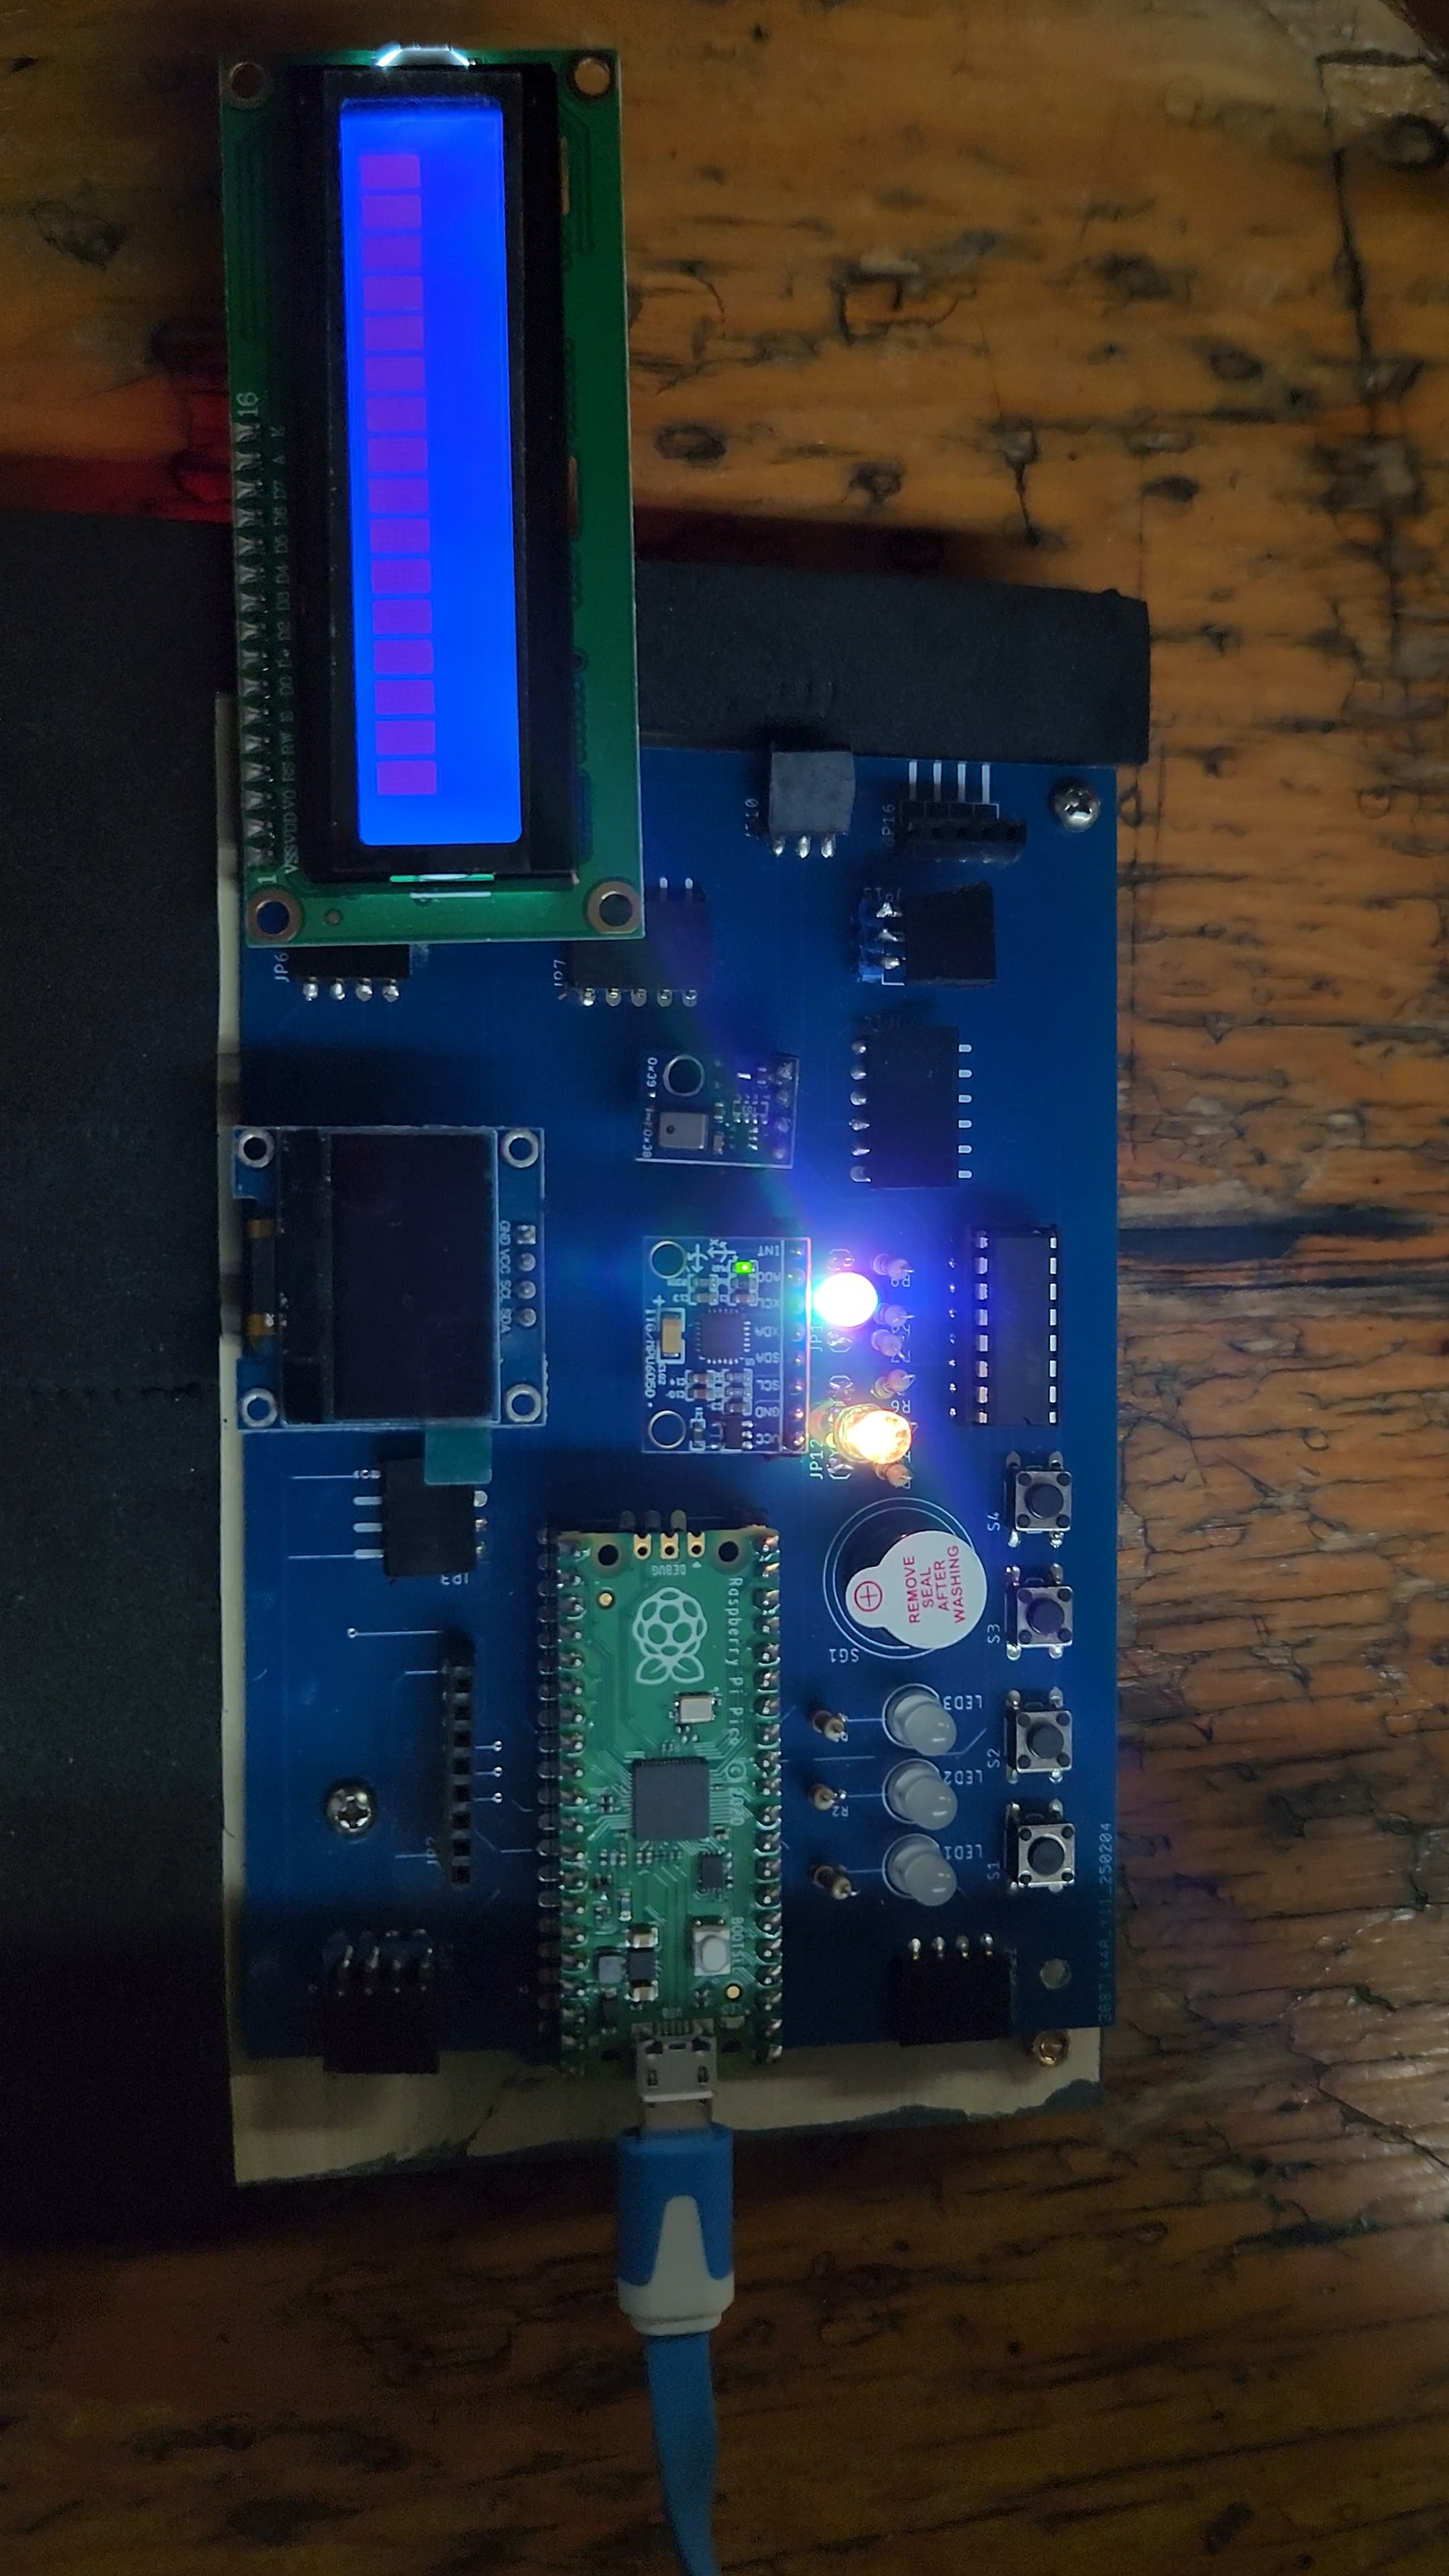
\includegraphics[width=0.25\textwidth, angle=90]{img/Actividad3/Act3_5.jpg}
        \caption{Secuencia en posición P4: el LED del pin P4 se activa con el valor \texttt{0b010000}, penúltimo paso de la secuencia ascendente.}
    \end{figure}

    \begin{figure}[H]
        \centering
        
\includegraphics[width=0.25\textwidth, angle=90]{img/Actividad3/Act3_6.jpg}
        \caption{Secuencia en posición P5: último LED de la secuencia encendido con el valor \texttt{0b100000}, antes de reiniciar el ciclo desde P0.}
    \end{figure}

    \subsection*{Análisis de resultados}

    Al ejecutar el programa, se comprobó que la secuencia generada coincide exactamente con el patrón descrito en la Tabla 10-1. Las Figuras 3 a 8 evidencian cómo cada LED del expansor PCF8574 se enciende de forma individual y secuencial, comenzando por el pin P0 y avanzando hasta el pin P5, para luego reiniciar el ciclo de manera continua. El comportamiento observado confirma que la escritura directa en el puerto del expansor mediante \texttt{pcf.port} permite controlar simultáneamente el estado de todos los pines de salida con un solo valor binario, lo cual resulta más eficiente que manipular cada pin de forma independiente. La comunicación I2C entre la Raspberry Pi Pico y el PCF8574 en la dirección \texttt{0x39} se mantuvo estable durante toda la ejecución, sin pérdida de datos ni errores de transmisión. El retardo de 0.5 segundos entre cada transición permitió apreciar claramente el desplazamiento del bit activo a través de los seis LEDs, generando un efecto visual de luz en movimiento que recorre los pines de menor a mayor peso. Como se observa en las imágenes, cada LED se enciende con un color específico del RGB del PCF8574, donde el color varía según el pin activo, lo que verifica que la asignación de pines y la polaridad de los LEDs están configuradas correctamente en el circuito. El resultado obtenido es el esperado y cumple con los requisitos de la actividad, demostrando el dominio del protocolo I2C para el control de dispositivos periféricos mediante el expansor de puertos.

    \newpage

    \section*{Actividad 4}

    \noindent Escribir el siguiente código; comentar y explicar su funcionamiento; se utilizará circuito de la actividad previa.

    \begin{lstlisting}[basicstyle=\ttfamily\footnotesize,caption={Figura 10-11. Código; actividad 4}]
    import pcf8574
    from machine import I2C, Pin
    import time

    i2c = I2C (0,scl=Pin(9), sda=Pin(8))
    pcf = pcf8574.PCF8574(i2c, 0x39)
    ON = 0
    OFF = 1
    pcf.port = 0x3F

    pcf.pin (6, 1)   #Entrada P6
    print("iniciamos")
    while True:
        if (pcf.pin(6)==0):
            pcf.pin(0,ON)
            print("Alto")
            pcf.pin (6, 1)
        else:
            pcf.pin(0,OFF)
            print("bajo")
            pcf.pin (6, 1)
    \end{lstlisting}
    
    \section*{Propuesta de solución}

    Para esta actividad se propone implementar un sistema de lectura de botón y control de LED utilizando el expansor PCF8574 como dispositivo de entrada y salida simultánea a través del bus I2C. La lógica invertida es fundamental en este circuito: dado que los pines del PCF8574 operan con resistencias de pull-up internas, un botón presionado genera un nivel lógico bajo (0) mientras que un botón sin presionar mantiene un nivel alto (1). Por esta razón, se definen las constantes \texttt{ON = 0} y \texttt{OFF = 1} para reflejar correctamente esta polaridad. El pin P6 se configura como entrada para leer el estado del botón, mientras que el pin P0 actúa como salida para controlar el LED. El valor inicial del puerto se establece en \texttt{0x37} (0b00110111) para configurar adecuadamente los pines de salida. Se utiliza un retardo de 0.1 segundos en el bucle principal para evitar la saturación del bus I2C y proporcionar un antirrebote básico por software, garantizando lecturas estables del botón.

    \begin{center}
    \scalebox{0.85}{
    \begin{tikzpicture}[node distance=1.05cm, every node/.style={font=\scriptsize}]
        \node (start) [startstop, text width=2.6cm] {Inicio};
        \node (import) [process, below=of start, text width=7.5cm] {Importar \texttt{pcf8574}, \texttt{I2C}, \texttt{Pin} y \texttt{time}.};
        \node (init) [process, below=of import, text width=7.5cm] {Inicializar I2C en SCL=9, SDA=8. Crear objeto PCF8574 en \texttt{0x39}.};
        \node (const) [process, below=of init, text width=5.5cm] {Definir \texttt{ON = 0}, \texttt{OFF = 1}.};
        \node (port) [process, below=of const, text width=5.5cm] {Establecer \texttt{pcf.port = 0x37}.};
        \node (print) [io, below=of port, text width=4.5cm] {Imprimir ``Iniciamos''.};
        \node (setinp) [process, below=of print, text width=5.5cm] {Configurar P6 como entrada: \texttt{pcf.pin(6, 1)}.};
        \node (check) [decision, below=of setinp, text width=3.5cm, aspect=2.5] {¿\texttt{pcf.pin(6)} == 0?};
        \node (ledon) [process, right=2.5cm of check, text width=4.5cm] {Encender LED: \texttt{pcf.pin(0, ON)}. Imprimir ``Bajo''.};
        \node (ledoff) [process, left=2.5cm of check, text width=4.5cm] {Apagar LED: \texttt{pcf.pin(0, OFF)}. Imprimir ``Alto''.};
        \node (delay) [process, below=2.0cm of check, text width=4.5cm] {Esperar 0.1 segundos.};

        \draw [arrow] (start) -- (import);
        \draw [arrow] (import) -- (init);
        \draw [arrow] (init) -- (const);
        \draw [arrow] (const) -- (port);
        \draw [arrow] (port) -- (print);
        \draw [arrow] (print) -- (setinp);
        \draw [arrow] (setinp) -- (check);
        \draw [arrow] (check.east) -- node[above, font=\scriptsize] {Sí} (ledon.west);
        \draw [arrow] (check.west) -- node[above, font=\scriptsize] {No} (ledoff.east);
        \draw [arrow] (ledon.south) |- (delay.east);
        \draw [arrow] (ledoff.south) |- (delay.west);
        \draw [arrow] (delay.south) -- ++(0,-0.5) -| ([xshift=-7.5cm]setinp.west) -- (setinp.west);
    \end{tikzpicture}
    }
    \end{center}

    El diagrama de flujo ilustra el funcionamiento del programa, que inicia con la configuración del hardware y la definición de las constantes de lógica invertida. Tras establecer el estado inicial del puerto e imprimir el mensaje de inicio, el programa entra en un bucle infinito donde primero configura el pin P6 como entrada de alta impedancia y luego evalúa su estado. Si el botón está presionado (nivel bajo), se enciende el LED en P0 y se imprime ``Bajo'' en la consola serial; en caso contrario, se apaga el LED y se imprime ``Alto''. Después de cada evaluación, se introduce un retardo de 100 milisegundos antes de reiniciar el ciclo. Este flujo garantiza una respuesta inmediata al cambio de estado del botón, demostrando la capacidad del PCF8574 para funcionar como dispositivo bidireccional en el bus I2C.

    \section*{Desarrollo}

    \lstinputlisting[language={[LAB]Python}, caption=Código de la Actividad 4, basicstyle=\ttfamily\scriptsize]{Code/Act4.py}

    \begin{figure}[H]
        \centering
        
\includegraphics[width=0.75\textwidth]{img/Actividad4/Act4_1.jpg}
        \caption{Botón S4 presionado: se observa el dedo presionando el botón conectado al pin P6 del PCF8574, lo que provoca que el LED en P0 se encienda en color rojo, confirmando la lectura de nivel bajo en la entrada.}
    \end{figure}

    \begin{figure}[H]
        \centering
        
\includegraphics[width=0.75\textwidth]{img/Actividad4/Act4_2.jpg}
        \caption{Botón S4 sin presionar: al liberar el botón, el pin P6 retorna a nivel alto por la resistencia de pull-up interna, apagando el LED en P0 y confirmando el funcionamiento correcto de la lógica invertida.}
    \end{figure}

    \subsection*{Análisis de resultados}

    La ejecución del programa demostró el correcto funcionamiento del expansor PCF8574 como dispositivo bidireccional a través del protocolo I2C. Como se observa en la Figura 9, al presionar el botón S4 conectado al pin P6, el LED conectado al pin P0 se enciende inmediatamente en color rojo, mientras que en la consola serial se imprime el mensaje ``Bajo'', indicando que el pin de entrada detectó un nivel lógico bajo. Por el contrario, la Figura 10 muestra que al soltar el botón, el LED se apaga y el mensaje ``Alto'' aparece en la consola, confirmando que la resistencia de pull-up interna del PCF8574 retorna el pin a su estado de reposo. La lógica invertida implementada con las constantes \texttt{ON = 0} y \texttt{OFF = 1} es correcta y necesaria porque el PCF8574 utiliza salidas de colector abierto: un nivel bajo en el pin permite que fluya corriente a través del LED hacia tierra, encendiéndolo, mientras que un nivel alto lo apaga. La reconfiguración del pin P6 como entrada dentro del bucle mediante \texttt{pcf.pin(6, 1)} es indispensable porque cada escritura en el puerto podría alterar el estado de dicho pin. El retardo de 0.1 segundos proporciona un antirrebote básico que evita lecturas erráticas durante la transición mecánica del botón. Los resultados obtenidos son los esperados y demuestran que el PCF8574 puede gestionar entradas y salidas de manera simultánea, ampliando las capacidades de E/S de la Raspberry Pi Pico mediante una comunicación I2C de solo dos líneas.

    \newpage
    \section*{Actividad 5}

    \noindent Escribir el siguiente código, comentar e indicar que hace, revisar las librerías empleadas.

    \begin{center}
        \resizebox{0.6\linewidth}{!}{
        \begin{tikzpicture}[>=latex]

            % 1. Dibujar Raspberry Pi Pico
            \begin{scope}[xshift=5cm, yshift=0cm]
                \picoboard
            \end{scope}

            % 2. Dibujar Módulo LCD I2C
            % Dibujado con borde azul como en la imagen
            \draw[very thick, blue!70!black] (-3, -4.6) rectangle (1.5, -5.7);
            \node[align=center, font=\large\sffamily\bfseries] at (-0.75, -5.15) {LCD I2C};
            
            % Textos de los pines del LCD
            \node[right, font=\small\sffamily\bfseries, text depth=0pt] at (-3, -4.85) {VCC};
            \node[right, font=\small\sffamily\bfseries, text depth=0pt] at (-3, -5.45) {GND};
            \node[left, font=\small\sffamily\bfseries, text depth=0pt] at (1.5, -4.95) {SDA};
            \node[left, font=\small\sffamily\bfseries, text depth=0pt] at (1.5, -5.40) {SCL};

            % -------------------------------------------------------------
            % RUTEOS (Coordenadas absolutas para evitar errores)
            % -------------------------------------------------------------

            % Conexiones de Alimentación del LCD
            % VCC a 5V (Cable Rojo, hacia arriba)
            \draw[red, very thick] (-2.5, -4.6) -- (-2.5, -3.8) node[vcc]{5V};

            % GND a Tierra (Cable Negro, hacia abajo)
            \draw[very thick] (-2.5, -5.7) -- (-2.5, -6.5) node[ground]{};

            % Conexiones I2C
            % SDA al pin P11 (GP8) - Cable Azul
            % El pin P11 de la Pico (xshift=5) está en x=4.6 absoluto
            \draw[blue, thick] (1.5, -4.95) -- (4.6, -4.95); 

            % SCL al pin P12 (GP9) - Cable Verde
            \draw[green!70!black, thick] (1.5, -5.40) -- (4.6, -5.40); 

        \end{tikzpicture}
        }
    \end{center}

    \begin{lstlisting}[basicstyle=\ttfamily\footnotesize,caption={Figura 10-12. Código ejemplo; LCD I2C}]
    from machine import I2C, Pin
    import time
    from esp8266_i2c_lcd import I2cLcd

    DEFAULT_I2C_ADDR = 0x27
    i2c = I2C(0,scl=Pin(9), sda=Pin(8), freq=200000)
    lcd = I2cLcd(i2c, DEFAULT_I2C_ADDR, 2, 16)

    lcd.putstr("UNAM!\nFI")
    time.sleep(3)
    lcd.clear()

    lcd.move_to(3, 0)
    lcd.putstr("Laboratorio")
    lcd.move_to(0, 1)
    lcd.putstr("* M I C R O S *")
    time.sleep(1)
    \end{lstlisting}

    \section*{Propuesta de solución}

    Para esta actividad se propone controlar una pantalla LCD de 16 columnas por 2 filas mediante el protocolo I2C, utilizando el módulo adaptador PCF8574 integrado en el módulo LCD I2C con dirección por defecto \texttt{0x27}. La librería \texttt{esp8266\_i2c\_lcd} proporciona una interfaz de alto nivel que abstrae la complejidad del controlador HD44780 del LCD, permitiendo escribir texto, limpiar la pantalla y posicionar el cursor con métodos sencillos. Se decide inicializar el bus I2C a una frecuencia de 200 kHz para garantizar la estabilidad de la comunicación con el módulo LCD. El programa se estructura en dos fases: primero muestra el texto ``UNAM!'' en la primera línea y ``FI'' en la segunda línea durante 3 segundos, y después limpia la pantalla para mostrar ``Laboratorio'' centrado en la primera línea y ``* MICROS*'' en la segunda. El uso de \texttt{lcd.move\_to(columna, fila)} permite posicionar el cursor en coordenadas específicas para centrar el texto visualmente, lo cual resulta más elegante que escribir espacios en blanco. Esta estrategia demuestra las capacidades fundamentales de la librería: escritura directa, limpieza de pantalla y posicionamiento del cursor.

    \textbf{Explicacion diagra de flujo:}

    El diagrama de flujo presenta un programa de ejecución lineal sin bucles, que sigue una secuencia de pasos bien definida. Tras la importación de las librerías y la inicialización del bus I2C con el objeto LCD, el programa escribe el primer mensaje utilizando el carácter de salto de línea \texttt{\textbackslash n} para distribuir el texto en ambas filas de la pantalla. Después de una pausa de 3 segundos que permite al usuario leer el mensaje, se ejecuta la limpieza completa del display. A continuación, se utiliza el método \texttt{move\_to} para posicionar el cursor en la columna 3 de la primera fila, logrando que el texto ``Laboratorio'' aparezca centrado, y luego en la columna 0 de la segunda fila para escribir ``* MICROS*''. El programa finaliza tras una espera de 1 segundo. Este flujo es correcto porque demuestra las operaciones fundamentales del LCD I2C: escritura con salto de línea automático, limpieza de pantalla, posicionamiento preciso del cursor y la capacidad de actualizar el contenido de la pantalla de manera dinámica.

    \begin{center}
    \scalebox{0.85}{
    \begin{tikzpicture}[node distance=1.05cm, every node/.style={font=\scriptsize}]
        \node (start) [startstop, text width=2.6cm] {Inicio};
        \node (import) [process, below=of start, text width=7.5cm] {Importar \texttt{I2C}, \texttt{Pin}, \texttt{time} y \texttt{I2cLcd}.};
        \node (init) [process, below=of import, text width=7.5cm] {Inicializar I2C en SCL=9, SDA=8 a 200 kHz. Crear objeto LCD (2 filas, 16 columnas) en \texttt{0x27}.};
        \node (write1) [process, below=of init, text width=5.5cm] {Escribir ``UNAM!\textbackslash nFI'' en la pantalla.};
        \node (wait1) [process, below=of write1, text width=4.5cm] {Esperar 3 segundos.};
        \node (clear) [process, below=of wait1, text width=4.5cm] {Limpiar la pantalla LCD.};
        \node (move1) [process, below=of clear, text width=6.0cm] {Mover cursor a columna 3, fila 0. Escribir ``Laboratorio''.};
        \node (move2) [process, below=of move1, text width=6.0cm] {Mover cursor a columna 0, fila 1. Escribir ``* MICROS*''.};
        \node (wait2) [process, below=of move2, text width=4.5cm] {Esperar 1 segundo.};
        \node (end) [startstop, below=of wait2, text width=2.6cm] {Fin};

        \draw [arrow] (start) -- (import);
        \draw [arrow] (import) -- (init);
        \draw [arrow] (init) -- (write1);
        \draw [arrow] (write1) -- (wait1);
        \draw [arrow] (wait1) -- (clear);
        \draw [arrow] (clear) -- (move1);
        \draw [arrow] (move1) -- (move2);
        \draw [arrow] (move2) -- (wait2);
        \draw [arrow] (wait2) -- (end);
    \end{tikzpicture}
    }
    \end{center}

    \section*{Desarrollo}

    \lstinputlisting[language={[LAB]Python}, caption=Código de la Actividad 5, basicstyle=\ttfamily\scriptsize]{Code/Act5.py}

    \begin{figure}[H]
        \centering
        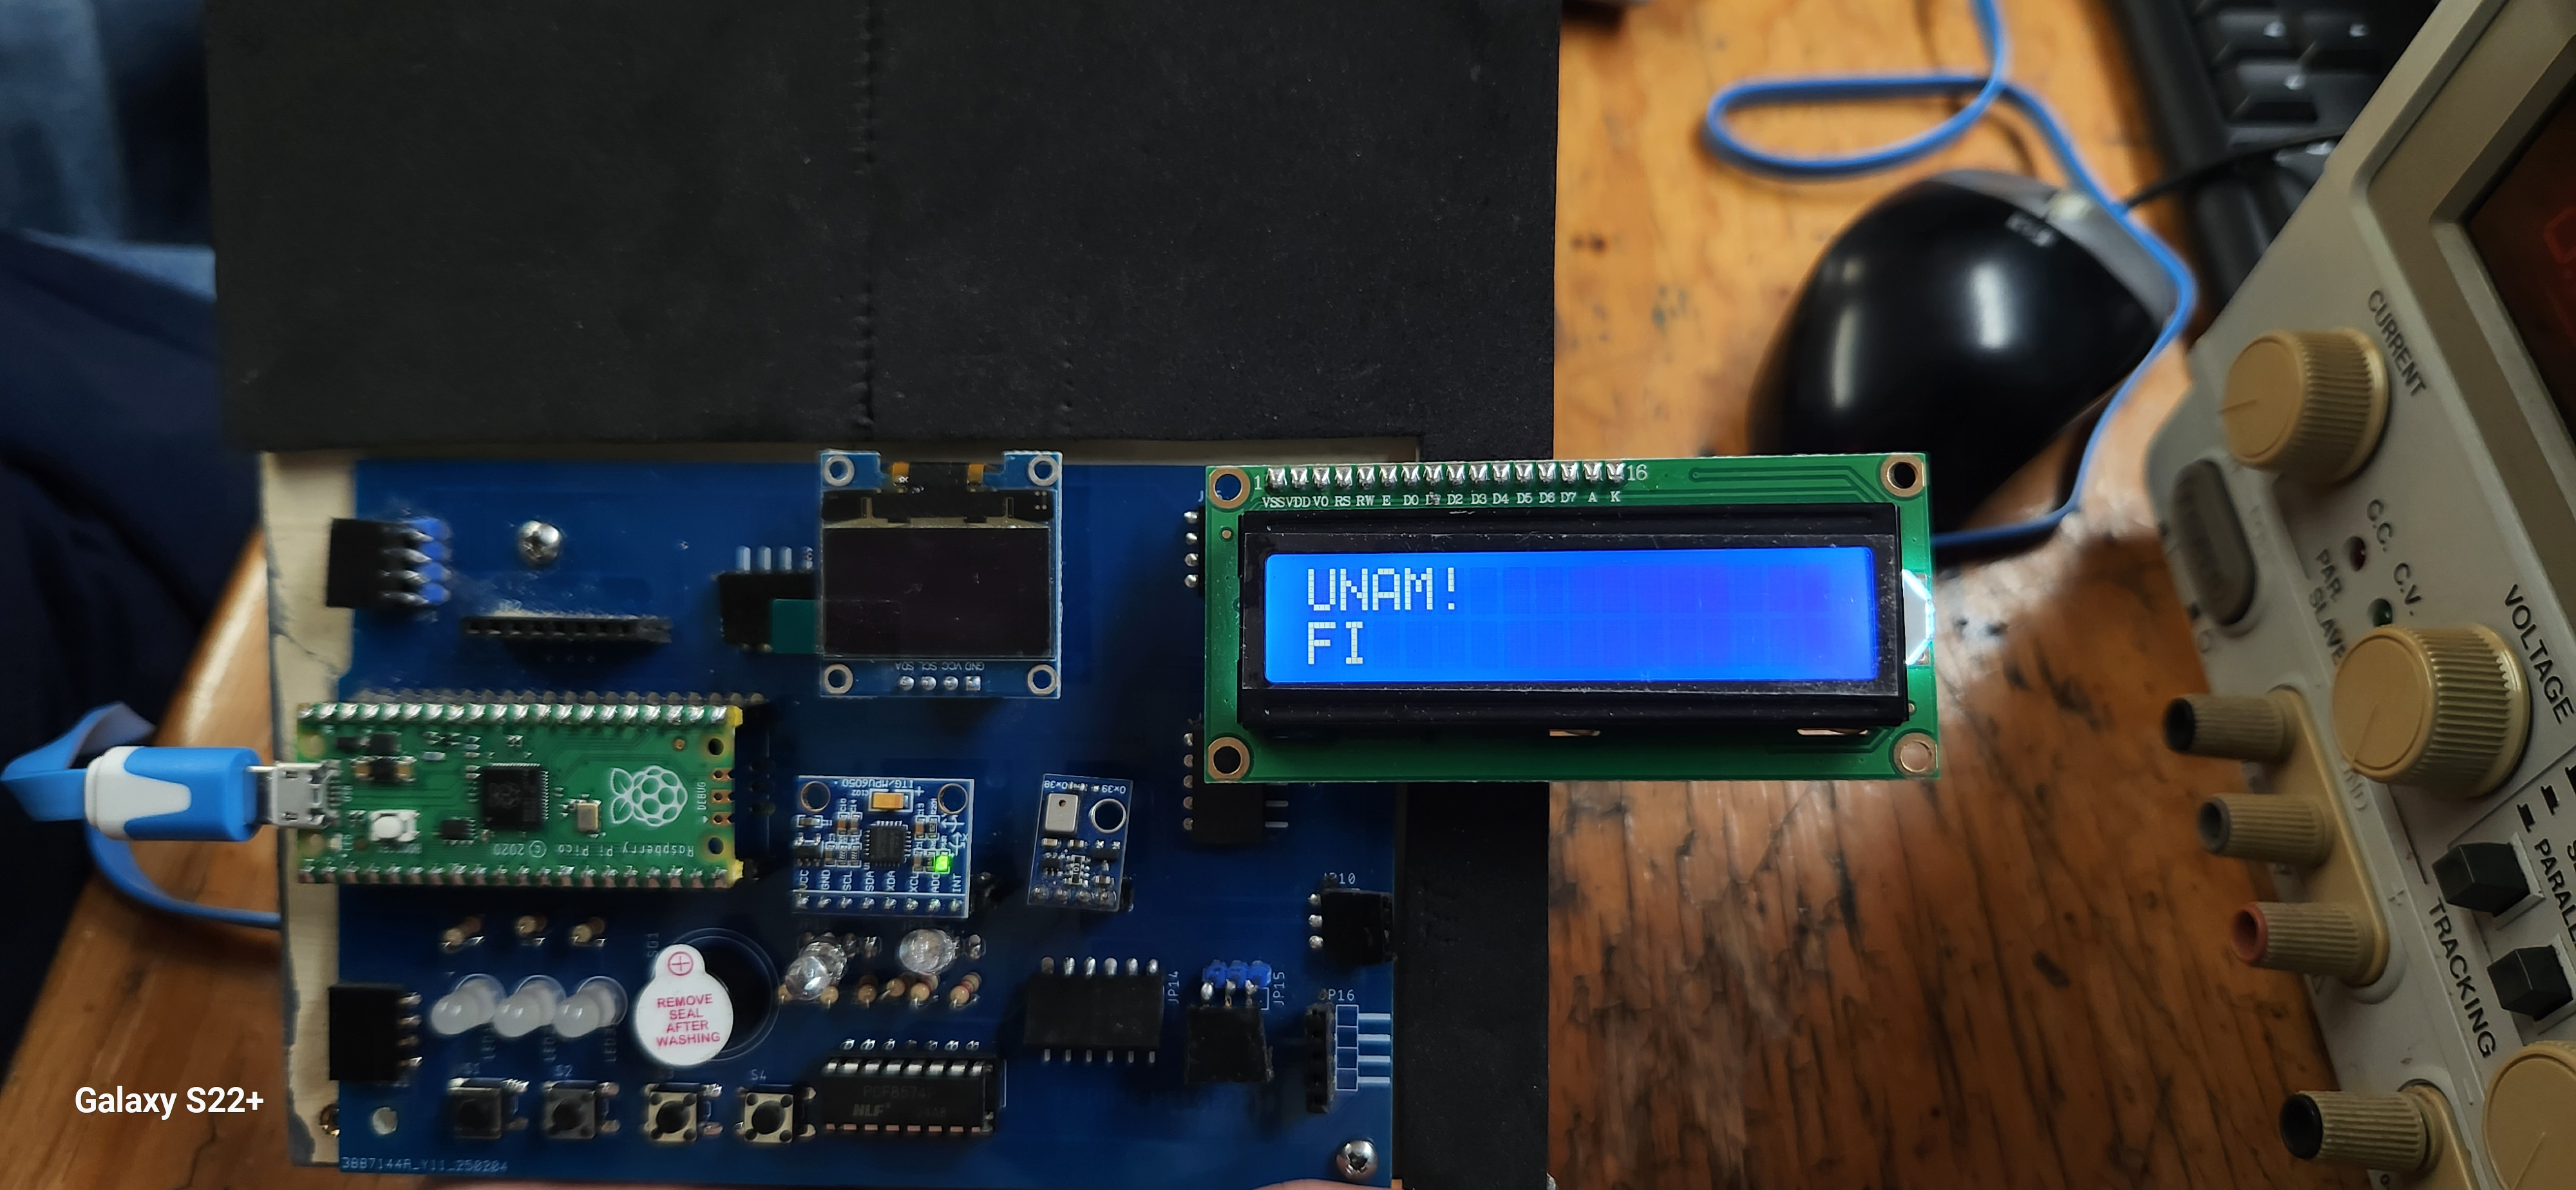
\includegraphics[width=0.75\textwidth]{img/Actividad5/Act5_2.jpg}
        \caption{Primera fase del programa: la pantalla LCD muestra ``UNAM!'' en la primera línea y ``FI'' en la segunda línea, correspondiente a la instrucción \texttt{lcd.putstr("UNAM!\textbackslash nFI")} ejecutada al inicio del programa.}
    \end{figure}

    \begin{figure}[H]
        \centering
        
\includegraphics[width=0.75\textwidth]{img/Actividad5/Act5_1.jpg}
        \caption{Segunda fase del programa: tras limpiar la pantalla, el LCD muestra ``Laboratorio'' centrado en la primera línea (posicionado en la columna 3) y ``* MICROS*'' en la segunda línea, verificando el correcto funcionamiento de \texttt{lcd.move\_to()} y \texttt{lcd.putstr()}.}
    \end{figure}

    \subsection*{Análisis de resultados}

    La ejecución del programa confirmó el correcto funcionamiento de la comunicación I2C entre la Raspberry Pi Pico y la pantalla LCD a través del módulo adaptador con dirección \texttt{0x27}. Como se aprecia en la Figura 11, la primera fase del programa muestra exitosamente los textos ``UNAM!'' y ``FI'' distribuidos en las dos líneas del display, lo cual demuestra que el carácter de escape \texttt{\textbackslash n} dentro de la función \texttt{putstr()} es interpretado correctamente por la librería \texttt{esp8266\_i2c\_lcd} para realizar el salto de línea automático sin necesidad de reposicionar el cursor manualmente. La Figura 12 evidencia la segunda fase, donde después de ejecutar \texttt{lcd.clear()} para borrar completamente el contenido anterior, el texto ``Laboratorio'' aparece centrado horizontalmente en la primera fila gracias al desplazamiento de 3 columnas aplicado con \texttt{lcd.move\_to(3, 0)}, y ``* MICROS*'' se muestra alineado a la izquierda en la segunda fila. La frecuencia de operación del bus I2C de 200 kHz resultó adecuada para mantener una comunicación estable con el módulo LCD, ya que frecuencias superiores podrían generar errores de transmisión debido a las capacitancias parásitas del cableado. Los resultados obtenidos son los esperados y comprueban que la librería \texttt{I2cLcd} abstrae correctamente el protocolo de comunicación del controlador HD44780 del LCD, permitiendo controlar un display de 16x2 caracteres con solo dos líneas del bus I2C (SDA y SCL) más la alimentación, lo que representa una reducción significativa en el número de pines GPIO necesarios comparado con la conexión directa en modo paralelo que requeriría al menos 6 líneas de datos.

\section*{Actividad 6}

\noindent Escribir el siguiente c\'odigo, comentar e indicar que hace, revisar la librer\'ia utilizada.

\begin{center}
    \resizebox{0.6\linewidth}{!}{
    \begin{tikzpicture}[>=latex]

        % 1. Dibujar Raspberry Pi Pico (Desplazada a la derecha)
        \begin{scope}[xshift=5cm, yshift=0cm]
            \picoboard
        \end{scope}

        % 2. Dibujar M\'odulo DISPLAY OLED
        \draw[very thick] (-2.5, -3.8) rectangle (0, -6.6);
        \node[above, font=\small\sffamily\bfseries] at (-1.25, -3.6) {DISPLAY OLED};
        
        % Textos de los pines del OLED alineados a la derecha de la caja
        \node[left, font=\small\sffamily, text depth=0pt] at (0, -4.45) {SCL};
        \node[left, font=\small\sffamily, text depth=0pt] at (0, -4.95) {SDA};
        \node[left, font=\small\sffamily, text depth=0pt] at (0, -5.45) {VCC};
        \node[left, font=\small\sffamily, text depth=0pt] at (0, -5.95) {GND};

        % -------------------------------------------------------------
        % RUTEOS
        % -------------------------------------------------------------

        % Conexiones I2C
        % SDA al pin GP8 - Cable Azul
        \draw[blue, thick] (0, -4.95) -- (4.6, -4.95); 

        % SCL al pin GP9 - Cable Verde
        \draw[green!70!black, thick] (0, -4.45) -| (2.8, -5.40) -- (4.6, -5.40); 

        % Conexiones de Alimentaci\'on
        % VCC a 3.3V (Cable Rojo)
        \draw[red, thick] (0, -5.45) -- (1.8, -5.45) -- (1.8, -5.8);
        \draw[very thick] (1.3, -5.8) -- (2.3, -5.8);
        \node[below, font=\small\sffamily\bfseries] at (1.8, -5.8) {3.3V};

        % GND a Tierra (Cable Gris)
        \draw[gray, thick] (0, -5.95) -- (0.8, -5.95) -- (0.8, -6.3);
        \node[ground] at (0.8, -6.3) {};

    \end{tikzpicture}
    }
    \end{center}

    \begin{lstlisting}[basicstyle=\ttfamily\footnotesize,caption={Figura 10-13. C\'odigo de prueba; actividad 6}]
    from machine import Pin, I2C
    from ssd1306 import SSD1306_I2C

    i2c = I2C(0, scl=Pin(9),sda=Pin(8),freq=400000)
    oled = SSD1306_I2C(128,64,i2c)

    devices = i2c.scan()
    if devices:
        for d in devices:
            print("I2C Adress: " + hex(d))

    oled.fill(0)
    oled.text("Microcomputadoras",1,6,1)
    oled.text("Practica I2C",3,30,1)
    oled.show()
    print("UNAM FI")
    \end{lstlisting}

    \section*{Propuesta de solución}

    El programa proporcionado inicializa el bus I2C en los pines GPIO 8 (SDA) y GPIO 9 (SCL) con una frecuencia de 400 kHz y se apoya de la librería \texttt{ssd1306} para controlar el display OLED, lo primero que se hace es escanear el bus I2C con \texttt{scan()} para detectar todos los dispositivos conectados, mostrando sus direcciones hexadecimales en la consola. Luego, se limpia la pantalla con \texttt{fill(0)}, se escriben dos textos ("Microcomputadoras" en (1,6) y "Practica I2C" en (3,30)) con color blanco (1), y paralelamente, se imprime el mensaje "UNAM FI" en la consola serial.

    \subsection*{Investigación de la librería \texttt{ssd1306}}

    La librería \texttt{ssd1306} para MicroPython permite controlar displays OLED basados en el controlador SSD1306, tanto en versión I2C como SPI. Sus principales características son:

    \begin{itemize}
        \item \texttt{SSD1306\_I2C(width, height, i2c, addr=0x3C)}: Constructor que recibe el ancho y alto del display (com\'unmente 128x64 o 128x32), el objeto I2C configurado y la direcci\'on I2C del dispositivo (por defecto 0x3C, aunque algunos displays usan 0x3D).
        \item \texttt{fill(c)}: Llena toda la pantalla con el valor especificado (0 para apagar p\'ixeles, 1 para encender).
        \item \texttt{text(string, x, y, c)}: Escribe una cadena de texto en la posici\'on (x, y) con el color especificado (0=negro, 1=blanco). La librer\'ia incluye una fuente interna de 8x8 p\'ixeles.
        \item \texttt{show()}: Transfiere el contenido del buffer interno al display f\'isico.
        \item \texttt{pixel(x, y, c)}: Permite dibujar un p\'ixel individual en coordenadas espec\'ificas.
        \item \texttt{scroll(dx, dy)}: Desplaza el contenido de la pantalla horizontal y verticalmente.
    \end{itemize}

    Esta librería nos ayuda a automatizar los comandos del controlador SSD1306 (como activaci\'on de display, configuraci\'on de contraste, direccionamiento de memoria), permitiendo al programador trabajar a nivel de abstracci\'on de p\'ixeles y texto.

    % Diagrama de flujo corregido
    \begin{center}
        \scalebox{0.85}{
        \begin{tikzpicture}[node distance=1.05cm, every node/.style={font=\scriptsize}]
            \node (start6) [startstop, text width=2.6cm] {Inicio};
            \node (init6) [process, below=of start6, text width=8.0cm] {Importar librerias: \texttt{Pin}, \texttt{I2C}, \texttt{SSD1306\_I2C}.};
            \node (config6) [process, below=of init6, text width=8.0cm] {Configurar I2C(0) con SDA=GP8, SCL=GP9, freq=400kHz. Crear objeto \texttt{oled} de 128x64.};
            \node (scan6) [process, below=of config6, text width=6.5cm] {Ejecutar \texttt{i2c.scan()} para detectar dispositivos I2C.};
            
            \node (decision6) [decision, below=of scan6, text width=3.5cm, aspect=2] {¿Hay dispositivos?};
            
            % Camino SI
            \node (print6) [process, below=1.2cm of decision6, text width=6.5cm] {Recorrer \texttt{devices} e imprimir direcciones hexadecimales.};
            
            % Camino NO
            \node (nofound6) [process, right=1.5cm of decision6, text width=4.5cm] {Imprimir "No se encontraron dispositivos".};
            
            % Bloques comunes (fuera del IF)
            \node (fill6) [process, below=1.2cm of print6, text width=4.5cm] {Limpiar pantalla con \texttt{oled.fill(0)}.};
            \node (text6) [process, below=of fill6, text width=7.0cm] {Escribir "Microcomputadoras" y "Practica I2C" con \texttt{oled.text()}.};
            \node (show6) [process, below=of text6, text width=4.5cm] {Actualizar display con \texttt{oled.show()} e imprimir "UNAM FI".};
            \node (end6) [startstop, below=of show6, text width=2.0cm] {Fin};
            
            % Dibujado de flechas principales
            \draw [arrow] (start6) -- (init6);
            \draw [arrow] (init6) -- (config6);
            \draw [arrow] (config6) -- (scan6);
            \draw [arrow] (scan6) -- (decision6);
            
            % Lógica condicional
            \draw [arrow] (decision6) -- node[right] {Si} (print6);
            \draw [arrow] (decision6) -- node[above] {No} (nofound6);
            
            % Unión de flujos hacia la sección de la OLED
            \draw [arrow] (print6) -- (fill6);
            \draw [arrow] (nofound6) |- (fill6); % El camino "No" se une antes de limpiar pantalla
            
            % Flujo final
            \draw [arrow] (fill6) -- (text6);
            \draw [arrow] (text6) -- (show6);
            \draw [arrow] (show6) -- (end6);
            
        \end{tikzpicture}
        }
    \end{center}
    \newpage

    \section*{Desarrollo}

    \lstinputlisting[language={[LAB]Python}, caption=C\'odigo de la Actividad 6, basicstyle=\ttfamily\scriptsize]{Code/Act6.py}

    \begin{figure}[H]
        \centering
        
\includegraphics[width=0.8\textwidth]{img/Actividad6/Act6_1.jpg}
        \caption{Mensajes en el display OLED SSD1306 controlado por la Raspberry Pi Pico mediante bus I2C.}
    \end{figure}

    \subsection*{Análisis de resultados}

    El programa logra inicializar correctamente el bus I2C a 400 kHz y detectar el display OLED en la direcci\'on 0x3C y el escaneo previo con \texttt{scan()} resulta \'util para verificar la conexi\'on antes de intentar escribir en el dispositivo y la pantalla muestra correctamente los textos "Microcomputadoras" en la coordenada (1,6) y "Practica I2C" en (3,30), además del mensaje "UNAM FI". La frecuencia de 400 kHz permite una actualizaci\'on r\'apida del display, aunque para el SSD1306 la velocidad t\'ipica es de 100 kHz (modo est\'andar), por lo que 400 kHz tambi\'en funciona correctamente en la mayor\'ia de los casos. Las funciones \texttt{fill(0)} y \texttt{show()} gestionan eficientemente el buffer de 1024 bytes (128x64/8) correspondiente a la memoria del display.

    \newpage
    \section*{Actividad 7}

    \noindent Escribir, comentar e indicar que hace el siguiente c\'odigo, este usa la comunicaci\'on I2C a trav\'es del m\'odulo TMP102 (sensor de temperatura).

    \begin{center}
    \resizebox{0.8\linewidth}{!}{
    \begin{tikzpicture}[>=latex]

        % 1. Dibujar Raspberry Pi Pico (Desplazada a la derecha)
        \begin{scope}[xshift=5cm, yshift=0cm]
            \picoboard % Asumiendo que esta macro define los nodos P11 para GP8 y P12 para GP9
        \end{scope}

        % 2. Dibujar Sensor de Temperatura TMP102
        \draw[thick, fill=white] (-3.0, -4.2) rectangle (0, -7.2);
        \node[above, font=\small\sffamily] at (-1.5, -4.2) {Sensor de Temperatura};
        \node[align=center, font=\small\sffamily] at (-1.5, -5.7) {TMP102};

        % Pines del lado Izquierdo del TMP102
        \foreach \y/\pin/\num in {-4.95/VCC/5, -6.75/GND/2} {
            \draw[red, thick] (-3.0, \y) -- (-3.4, \y) coordinate (T\pin);
            \node[right, font=\tiny\sffamily] at (-3.0, \y) {\pin};
            \node[above right, font=\tiny\sffamily, inner sep=1pt] at (T\pin) {\num};
        }

        % Pines del lado Derecho del TMP102
        \foreach \y/\pin/\num in {-4.95/SDA/6, -5.40/SCL/1, -6.30/ALERT/3, -6.75/ADD0/4} {
            \draw[red, thick] (0, \y) -- (0.4, \y) coordinate (T\pin);
            \node[left, font=\tiny\sffamily] at (0, \y) {\pin};
            \node[above left, font=\tiny\sffamily, inner sep=1pt] at (T\pin) {\num};
        }

        % -------------------------------------------------------------
        % RUTEOS CORREGIDOS
        % -------------------------------------------------------------

        % Conexiones I2C directas a los pines de la Pico
        % SDA al pin GP8 (P11 en la macro de la Pico)
        \draw[blue, thick] (TSDA) -- ++(1.0, 0) |- (P11); 

        % SCL al pin GP9 (P12 en la macro de la Pico)
        \draw[green!70!black, thick] (TSCL) -- ++(0.7, 0) |- (P12); 

        % Dirección I2C: Para que sea 0x48, ADD0 debe ir a GND
        \draw[thick] (TADD0) -- ++(0.2, 0) -- ++(0, -0.2) node[ground, scale=0.5]{};

        % Alimentación
        \draw[red, thick] (TVCC) -- (-4.2, -4.95) node[vcc]{3.3V};
        \draw[thick] (TGND) -- (-4.2, -6.75) node[ground]{};

    \end{tikzpicture}
    }
\end{center}

    \begin{lstlisting}[basicstyle=\ttfamily\footnotesize,caption={Figura 10-14. C\'odigo de ejemplo; actividad 7}]
    from machine import Pin, I2C
    import time

    i2c = I2C(0, scl=Pin(9), sda=Pin(8), freq=100000)
    addr = i2c.scan()
    print( "address is :" + str(addr) )

    for i in range(100):
        data = []
        data = i2c.readfrom(0x48, 2)
        intdata = int.from_bytes(data, 'big')
        tmp = intdata >> 4
        print(tmp * 0.0625)
        time.sleep(1)
    \end{lstlisting}

    \section*{Propuesta de soluci\'on}

    El programa proporcionado inicializa el bus I2C en los pines GPIO 8 (SDA) y GPIO 9 (SCL) con una frecuencia de 100 kHz, adecuada para el sensor TMP102. En un bucle de 100 iteraciones, lee 2 bytes desde la direcci\'on 0x48 (direcci\'on fija del TMP102 cuando ADD0 est\'a a GND). Los 2 bytes contienen la temperatura codificada en formato de 12 bits justificados a la izquierda. Se convierten los bytes a entero big-endian, se desplazan 4 bits a la derecha para obtener el valor de 12 bits, y se multiplica por 0.0625 (resoluci\'on de 0.0625°C por bit) y finalmente, se imprime la temperatura en grados Celsius y se espera 1 segundo antes de la siguiente lectura.

    \subsection*{Investigaci\'on del sensor TMP102}

    El TMP102 es un sensor de temperatura digital de alta precisi\'on de Texas Instruments que utiliza el bus I2C. Sus principales caracter\'isticas son:

    \begin{itemize}
        \item \textbf{Rango de medici\'on}: -40°C a +125°C
        \item \textbf{Precisi\'on}: ±0.5°C t\'ipica en el rango de -25°C a +85°C
        \item \textbf{Resoluci\'on}: 12 bits (0.0625°C por bit), configurable a 9, 10, 11 o 12 bits
        \item \textbf{Direcci\'on I2C}: 0x48 (con ADD0 a GND), 0x49 (ADD0 a VCC), 0x4A (ADD0 a SDA), 0x4B (ADD0 a SCL)
        \item \textbf{Formato de datos}: Los 12 bits de temperatura est\'an justificados a la izquierda en los 2 bytes de lectura. El bit 15 es el signo, los bits 14-4 son el valor entero, y los bits 3-0 son la parte fraccionaria (0.0625°C por bit). F\'ormula: Temperatura = (valor\_12bits) × 0.0625
        \item \textbf{Consumo}: 10 µA en modo activo, 1 µA en modo shutdown
    \end{itemize}

    % Diagrama de flujo compacto para TMP102
\begin{center}
    \scalebox{0.75}{ % Reducido un poco más para asegurar espacio
    \begin{tikzpicture}[node distance=0.6cm, every node/.style={font=\scriptsize}]
        \node (start) [startstop, text width=2.2cm] {Inicio};
        \node (init) [process, below=of start, text width=7.0cm] {Importar librerías: \texttt{Pin}, \texttt{I2C}, \texttt{time}.};
        \node (config) [process, below=of init, text width=7.0cm] {Configurar I2C(0) con SDA=GP8, SCL=GP9, freq=100kHz.};
        \node (scan) [process, below=of config, text width=6.0cm] {Ejecutar \texttt{i2c.scan()} para detectar dispositivos.};
        
        % Decisión con más espacio respecto a los bloques inferiores
        \node (decision) [decision, below=0.8cm of scan, text width=3.0cm, aspect=2] {¿Hay dispositivos?};
        
        % Bloque SI (Abajo)
        \node (print_addr) [process, below=0.8cm of decision, text width=6.0cm] {Imprimir dirección del dispositivo encontrado.};
        
        % Bloque NO (Derecha)
        \node (nofound) [process, right=1.2cm of decision, text width=4.0cm] {Imprimir "No se encontraron dispositivos".};
        
        % Bucle For
        \node (loop) [process, below=of print_addr, text width=5.0cm] {\texttt{for i in range(100)}: Iniciar bucle.};
        \node (read) [process, below=of loop, text width=6.0cm] {Leer 2 bytes desde dirección \texttt{0x48} con \texttt{i2c.readfrom()}.};
        \node (calc) [process, below=of read, text width=7.0cm] {Convertir bytes a entero, desplazar 4 bits y multiplicar por 0.0625.};
        \node (print_temp) [process, below=of calc, text width=5.0cm] {Imprimir temperatura calculada.};
        \node (sleep) [process, below=of print_temp, text width=4.0cm] {Esperar 1 segundo con \texttt{time.sleep(1)}.};
        
        \node (end) [startstop, below=0.8cm of sleep, text width=2.0cm] {Fin};

        % Flechas principales
        \draw [arrow] (start) -- (init);
        \draw [arrow] (init) -- (config);
        \draw [arrow] (config) -- (scan);
        \draw [arrow] (scan) -- (decision);
        
        % Lógica condicional
        \draw [arrow] (decision) -- node[right] {Si} (print_addr);
        \draw [arrow] (decision) -- node[above] {No} (nofound);
        
        % El camino "No" baja hacia el fin
        \draw [arrow] (nofound) |- (end.east);
        
        % Flujo del bucle
        \draw [arrow] (print_addr) -- (loop);
        \draw [arrow] (loop) -- (read);
        \draw [arrow] (read) -- (calc);
        \draw [arrow] (calc) -- (print_temp);
        \draw [arrow] (print_temp) -- (sleep);
        
        % Retorno del bucle (sale de sleep y entra a loop)
        \draw [arrow] (sleep.west) -- ++(-2.5,0) |- (loop.west);
        
        % Salida del bucle tras 100 iteraciones
        \draw [arrow] (sleep) -- (end);

    \end{tikzpicture}
    }
\end{center}

    \section*{Desarrollo}

    \lstinputlisting[language={[LAB]Python}, caption=C\'odigo de la Actividad 7, basicstyle=\ttfamily\scriptsize]{Code/Act7.py}

    \begin{figure}[H]
        \centering
        
\includegraphics[width=0.85\textwidth]{img/Actividad7/Act7_1.jpg}
        \caption{Lecturas del sensor TMP102.}
    \end{figure}

    \subsection*{An\'alisis de resultados}

    El programa logra inicializar correctamente el bus I2C a 100 kHz y detectar el sensor TMP102 en la direcci\'on 0x48. Las lecturas de temperatura obtenidas (aproximadamente 28.9°C a 30.9°C) son coherentes con la temperatura ambiente del laboratorio donde las variaciones corresponden a una prueba de funcionamiento del sensor donde le traspasamos nuestro calor y vimos un aumento de temperatura consistente. El c\'alculo de temperatura mediante desplazamiento de bits (tmp = intdata >> 4) y multiplicaci\'on por 0.0625 demuestra una correcta interpretaci\'on del formato de 12 bits justificados a la izquierda del TMP102. Las lecturas muestran una resoluci\'on de 0.0625°C (evidente en valores como 28.9375, 30.0625, 30.5625), validando la precisi\'on del m\'etodo de conversi\'on. 

    \newpage
    \section*{Actividad 8}

    \noindent  Escribir, comentar e indicar que hace el siguiente código, este usa la comunicación I2C a través del módulo AHT10 (sensor de temperatura y humedad); estudiar la librería empleada.

    \begin{center}
        \resizebox{0.8\linewidth}{!}{
        \begin{tikzpicture}[>=latex]

            % 1. Dibujar Raspberry Pi Pico (Desplazada a la derecha)
            \begin{scope}[xshift=5cm, yshift=0cm]
                \picoboard
            \end{scope}

            % 2. Dibujar Módulo Sensor AHT10
            \draw[thick] (-3, -3.5) rectangle (0, -6.5);

            % Textos descriptivos a la izquierda (Azul, Cursiva, Negrita)
            \node[align=center, font=\Large\sffamily\bfseries\itshape, text=blue!40!black] at (-6.5, -4.5) {Sensor de\\[0.1cm]Temperatura\\[0.1cm]y Humedad\\[0.1cm]AHT10};

            % Etiquetas de pines dentro del módulo
            \node[left, font=\normalsize\sffamily\bfseries\itshape] at (0, -4.95) {SDA};
            \node[left, font=\normalsize\sffamily\bfseries\itshape] at (0, -5.40) {SCL};
            \node[below, font=\normalsize\sffamily\bfseries\itshape] at (-0.8, -3.5) {VCC};
            \node[above, font=\normalsize\sffamily\bfseries\itshape] at (-0.8, -6.5) {GND};

            % -------------------------------------------------------------
            % RUTEOS (Coordenadas absolutas limpias)
            % -------------------------------------------------------------

            % Conexiones I2C (Directas horizontales)
            % SDA al pin P11 (GP8) - Cable Azul
            \draw[blue!80!black, very thick] (0, -4.95) -- (4.6, -4.95);
            % SCL al pin P12 (GP9) - Cable Verde
            \draw[green!60!black, very thick] (0, -5.40) -- (4.6, -5.40);

            % Conexiones de Alimentación
            % VCC a 3.3V (Cable Rojo -> Verde -> 3.3V)
            \draw[red, very thick] (-0.8, -3.5) -- (-0.8, -2.8);
            \draw[green!70!black, thick] (-0.8, -2.8) -- (-0.8, -2.5);
            \draw[thick] (-1.3, -2.5) -- (-0.3, -2.5); % Barra horizontal del 3.3V
            \node[above, font=\small\sffamily] at (-0.8, -2.5) {3.3V};

            % GND a Tierra (Cable Negro -> Verde -> Ground)
            \draw[black, very thick] (-0.8, -6.5) -- (-0.8, -7.2);
            \draw[green!70!black, thick] (-0.8, -7.2) -- (-0.8, -7.6);
            \node[ground] at (-0.8, -7.6) {}; % Símbolo de tierra estándar

        \end{tikzpicture}
        }
    \end{center}

    \begin{lstlisting}[basicstyle=\ttfamily\footnotesize,caption={Figura 10-15. Código de ejemplo; actividad 8}]
    import utime
    from machine import Pin, I2C
    import ahtx0

    i2c =I2C(0,sda=Pin(8),scl=Pin(9),freq=400000)
    sensor = ahtx0.AHT10(i2c)

    while True:
        print("\nTemperature: %0.2f C" % sensor.temperature)
        print("Humidity: %0.2f %%" % sensor.relative_humidity)
        utime.sleep(5)
    \end{lstlisting}
    \section*{Propuesta de solución}

    Dado que en esta aplicación se hace uso del módulo \texttt{AHT10} es necesario usar la biblioteca \texttt{ahtx0}.

    Sin embargo en el programa lo primero que se realiza es importar la biblioteca \texttt{utime} esto para poder realizar un retraso de entre lecturas, posteriormente se importan las clases \texttt{Pin} e \texttt{I2C} de la biblioteca \texttt{machine} para configurar la comunicación I2C, y finalmente se importa la clase \texttt{AHT10} de la biblioteca \texttt{ahtx0} para interactuar con el sensor.

    Una vez que ya se realizan las importaciones necesarias, se configura el bus I2C utilizando el puerto 0 de la Raspberry Pi Pico, con SDA en el pin GPIO 8 y SCL en el pin GPIO 9, a una frecuencia de 400 kHz. 

    Ya con el canal de comunicación configurado, se crea una instancia del sensor AHT10 pasando el objeto I2C como argumento, cuando se crea esta instancia, la biblioteca \texttt{ahtx0} se encarga de inicializar el sensor y prepararlo para las lecturas. De forma que \texttt{ahtx0} envía un comadno de inicialización al sensor AHT10, el cual realiza una calibración interna y se pone listo para medir temperatura y humedad. En caso de que no se pueda inicializar correctamente, la biblioteca lanzará una excepción que se puede manejar para detectar problemas de conexión o hardware.

    Mediante un bucle infinito, se imprimen en la consola los valores de temperatura y humedad obtenidos del sensor utilizando las propiedades \texttt{temperature} y \texttt{relative\_humidity} respectivamente. La biblioteca \texttt{ahtx0} se encarga de convertir registros complejos en propeidades simples, de forma que cuiando se llama al método \texttt{temperature}, la biblioteca envía el comando de medición, donde lee 6 bytes de datros, extrae los bits correspondientes a la temperatura y aplica la fórmula matemática. Para la propiedad \texttt{relative\_humidity}, la biblioteca realiza un proceso similar, pero extrayendo los bits correspondientes a la humedad y aplicando su fórmula de conversión escalando el valor a un porcentaje. Finalmente, se imprimen los valores que sew recuperaron y se realiza un retraso de 5 segundos antes de la siguiente lectura utilizando \texttt{utime.sleep(5)}.
    
    \newpage

    \begin{figure}[H]
        \begin{tikzpicture}[
            node distance=0.6cm, 
            every node/.style={font=\scriptsize},
            startstop/.style={rectangle, rounded corners, minimum width=2.2cm, minimum height=0.8cm, text centered, draw=black, fill=red!30},
            process/.style={rectangle, minimum width=3cm, minimum height=0.8cm, text centered, draw=black, fill=orange!20},
            decision/.style={diamond, aspect=2, minimum width=3cm, minimum height=1cm, text centered, draw=black, fill=green!20},
            arrow/.style={thick, ->, >=Stealth}
        ]

            % Nodos iniciales y de configuración
            \node (start) [startstop, text width=2.2cm] {Inicio};
            \node (init) [process, below=of start, text width=7.0cm] {Importar librerías: \texttt{utime}, \texttt{Pin}, \texttt{I2C}, \texttt{ahtx0}.};
            \node (config) [process, below=of init, text width=7.0cm] {Inicializar I2C(0) con SDA=Pin(8), SCL=Pin(9), freq=400kHz.};
            \node (sensor) [process, below=of config, text width=6.0cm] {Crear objeto sensor \texttt{ahtx0.AHT10(i2c)}.};
            
            % Bucle infinito
            \node (loop) [process, below=of sensor, text width=5.0cm] {Bucle infinito: \texttt{while True}};
            \node (print_temp) [process, below=of loop, text width=6.0cm] {Imprimir temperatura en $^\circ$C.};
            \node (print_hum) [process, below=of print_temp, text width=6.0cm] {Imprimir humedad relativa en \%.};
            \node (sleep) [process, below=of print_hum, text width=5.0cm] {Esperar 5 segundos con \texttt{utime.sleep(5)}.};

            % Flechas de flujo principal
            \draw [arrow] (start) -- (init);
            \draw [arrow] (init) -- (config);
            \draw [arrow] (config) -- (sensor);
            \draw [arrow] (sensor) -- (loop);
            \draw [arrow] (loop) -- (print_temp);
            \draw [arrow] (print_temp) -- (print_hum);
            \draw [arrow] (print_hum) -- (sleep);
            
            % Retorno del bucle infinito (sale del sleep y entra de nuevo al loop)
            \draw [arrow] (sleep.west) -- ++(-2.5,0) |- (loop.west);

        \end{tikzpicture}
        \centering
        \caption{Diagrama de flujo del programa para el sensor AHT10.}        
    \end{figure}


    \section*{Desarrollo}

    \lstinputlisting[language={[LAB]Python}, caption=Código de la Actividad 8, basicstyle=\ttfamily\scriptsize]{Code/Act8.py}

    \begin{figure}[H]
        \centering
        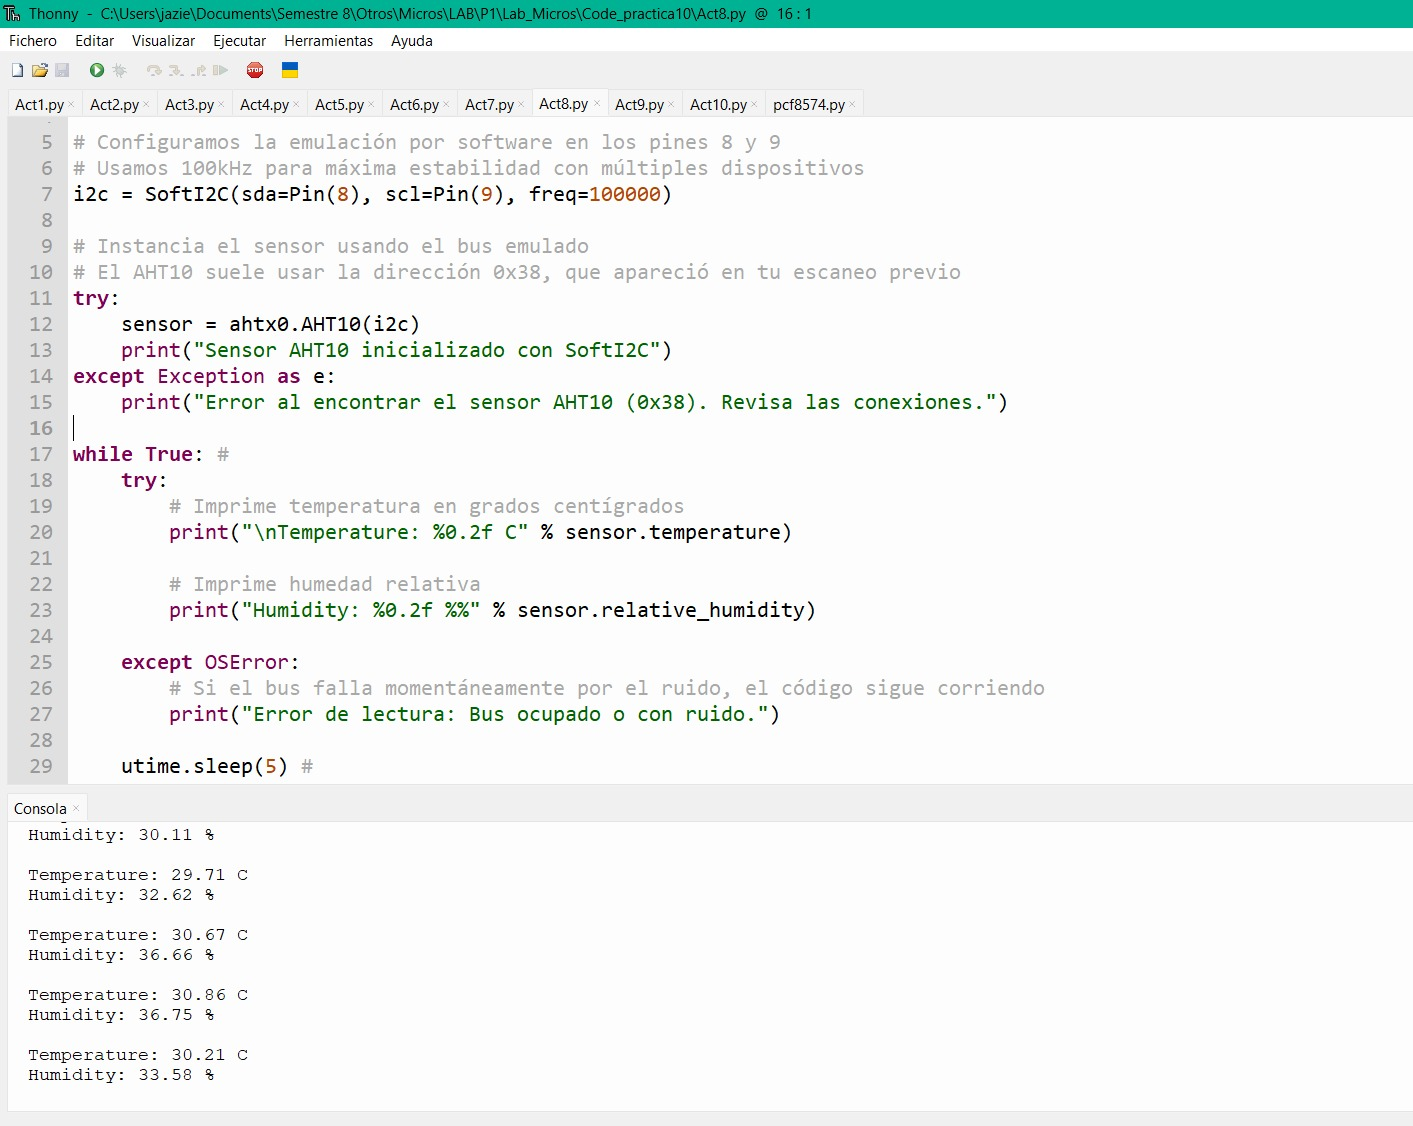
\includegraphics[width=0.85\textwidth]{img/Actividad8/Act8_1.jpg}
        \caption{Lecturas del sensor AHT10.}
    \end{figure}


    \subsection*{Análisis de resultados}

    A partir de cargar el código en la Raspberry Pi Pico, se observa que el programa logra inicializar correctamente el bus I2C a 400 kHz y crear una instancia del sensor AHT10 sin errores, lo que indica que la comunicación con el sensor es exitosa. Las lecturas de temperatura son correctas ya que en un inicio son de aproximadamente 29.71$^\circ C$, y al colocar la mano sobre el sensor, la temperatura aumenta a alrededor de 30.86$^\circ C$, lo que es consistente con el aumento de temperatura esperado debido al calor corporal. Las lecturas de humedad relativa también son coherentes, mostrando un valor inicial de aproximadamente 32.62\% y aumentando a cerca de 36.75\% al colocar la mano, lo que refleja el aumento de humedad debido al contacto directo con el sensor. 

    \section*{Actividad 9}

    \noindent MPU6050 Acelerómetro giroscopio.

    \begin{center}
        \resizebox{0.8\linewidth}{!}{
        \begin{tikzpicture}[>=latex]

            % 1. Dibujar Raspberry Pi Pico (Desplazada a la derecha)
            \begin{scope}[xshift=5cm, yshift=0cm]
                \picoboard
            \end{scope}

            % 2. Dibujar Módulo MPU 6050
            \draw[very thick, fill=white] (-4.0, -3.1) rectangle (-1.5, -7.2);
            
            % Títulos del módulo
            \node[above, font=\small\sffamily] at (-4.0, -2.9) {Giroscopio - Acelerómetro};
            \node[align=center, font=\small\sffamily] at (-2.75, -5.1) {MPU\\[0.1cm]6050\\[0.1cm](GY-521)};

            % Nombres de los pines alineados a la izquierda del borde derecho de la caja
            \foreach \y/\pin in {-3.60/VCC, -4.05/GND, -4.50/SCL, -4.95/SDA, -5.40/XDA, -5.85/XCL, -6.30/AD0, -6.75/INT} {
                \node[left, font=\tiny\sffamily, text depth=0pt, text=gray!80!black] at (-1.5, \y) {\pin};
            }

            % Conectores cortos (Stubs) saliendo del módulo con sus colores originales
            \draw[red, thick] (-1.5, -3.60) -- (-1.1, -3.60) coordinate (MVCC);
            \draw[red, thick] (-1.5, -4.05) -- (-1.1, -4.05) coordinate (MGND);
            \draw[green!70!black, thick] (-1.5, -4.50) -- (-1.1, -4.50) coordinate (MSCL);
            \draw[green!70!black, thick] (-1.5, -4.95) -- (-1.1, -4.95) coordinate (MSDA);
            
            % Pines no conectados
            \draw[red, thick] (-1.5, -5.40) -- (-1.1, -5.40); % XDA
            \draw[red, thick] (-1.5, -5.85) -- (-1.1, -5.85); % XCL
            \draw[red, thick] (-1.5, -6.30) -- (-1.1, -6.30); % AD0
            \draw[red, thick] (-1.5, -6.75) -- (-1.1, -6.75); % INT

            % -------------------------------------------------------------
            % RUTEOS (Limpios y ortogonales)
            % -------------------------------------------------------------

            % VCC a 3.3V (Sube desde el stub)
            \draw[green!70!black, thick] (MVCC) -- (-1.1, -2.5);
            \draw[very thick] (-1.6, -2.5) -- (-0.6, -2.5); % Barra horizontal del 3.3V
            \node[above, font=\small\sffamily] at (-1.1, -2.5) {3.3V};

            % GND a Tierra (Baja ordenadamente a un símbolo de tierra estándar)
            \draw[green!70!black, thick] (MGND) -- (-0.5, -4.05) -- (-0.5, -5.5);
            \node[ground] at (-0.5, -5.5) {};

            % Conexiones I2C
            % SDA al pin P11 (GP8) - Cable Azul (Alineación perfecta, ruta directa horizontal)
            \draw[blue!80!black, thick] (MSDA) -- (4.6, -4.95);

            % SCL al pin P12 (GP9) - Cable Verde (Ruteo ortogonal a 90° para evitar cruces sucios)
            \draw[green!70!black, thick] (MSCL) -- (1.5, -4.50) -- (1.5, -5.40) -- (4.6, -5.40);

        \end{tikzpicture}
        }
    \end{center}

    \begin{lstlisting}[basicstyle=\ttfamily\footnotesize,caption={Figura 10-16. Programa de ejemplo; actividad 9}]
    from imu import MPU6050
    from machine import Pin,I2C
    import utime

    i2c =I2C(0,sda=Pin(8),scl=Pin(9),freq=400000)
    imu = MPU6050(i2c)

    while True:
        ax =round(imu.accel.x,2)
        print(ax)
        utime.sleep_ms(200)
    \end{lstlisting}
    \section*{Propuesta de solución}

    El codigo que se proporciona es un programa básico para leer los datos del acelerómetro del sensor MPU6050 utilizando la comunicación I2C. 

    El programa comienza importando la clase \texttt{MPU6050} de la biblioteca \texttt{imu}, así como las clases \texttt{Pin} e \texttt{I2C} de la biblioteca \texttt{machine} para configurar la comunicación I2C, y la biblioteca \texttt{utime} para manejar los retrasos entre lecturas.

    De igual mane4ra que en la actividad anterior, se configura el bus I2C utilizando el puerto 0 de la Raspberry Pi Pico, con SDA en el pin GPIO 8 y SCL en el pin GPIO 9, a una frecuencia de 400 kHz. Luego, se crea una instancia del sensor MPU6050 pasando el objeto I2C como argumento, lo que inicializa el sensor y lo prepara para las lecturas.

    Cuadno se crea la instancia del sensor, la biblioteca \texttt{imu} se encarga de mapear los registros internos del sensor. Cuando se crea el objeto, la biblioteca configura el sensor para qu esté en modo activo y define el rango de sensibilidad del acelerómetro. Esto implica escribir en los registros de configuración del MPU6050 para habilitar el acelerómetro y establecer su rango de medición (por ejemplo, $\pm 2g$, $\pm 4g$, etc.).

    Por medio de un bucle infinito, el programa lee el valor del eje X del acelerómetro utilizando la propiedad \texttt{imu.accel.x}, que devuelve la aceleración en g's. La propiedad \texttt{accel} es un objeto que contiene las lecturas de los tres ejes del acelerómetro (X, Y, Z), y al acceder a \texttt{imu.accel.x}, la biblioteca ejecuta internamente una lectura de I2C, donde toma los dos bytes crudos del sensor, los combina y los dividfe por un factor de escala para convertirlos a unidades de g's. Por medio de la función \texttt{round()}, se redondea el valor a dos decimales para facilitar su lectura, y luego se imprime en la consola. Finalmente, se realiza un retraso de 200 milisegundos antes de la siguiente lectura utilizando \texttt{utime.sleep\_ms(200)}.

    \newpage

    \begin{figure}[H]
        \centering
        \begin{tikzpicture}[
            node distance=0.8cm and 0cm, 
            every node/.style={font=\small},
            % Estilos proporcionados
            startstop/.style={rectangle, rounded corners, minimum width=3cm, minimum height=1cm, text centered, draw=black, fill=red!30},
            process/.style={rectangle, minimum width=3cm, minimum height=1cm, text centered, draw=black, fill=orange!30},
            decision/.style={diamond, aspect=2, minimum width=3cm, minimum height=1cm, text centered, draw=black, fill=green!30},
            io/.style={trapezium, trapezium left angle=70, trapezium right angle=110, minimum width=3cm, minimum height=1cm, text centered, draw=black, fill=blue!30},
            arrow/.style={thick, ->, >=stealth}
        ]

            % Definición de los nodos
            \node (start) [startstop] {Inicio};
            \node (import) [process, below=of start, text width=6cm] {Importar librerías:\\ \texttt{MPU6050}, \texttt{Pin}, \texttt{I2C}, \texttt{utime}};
            \node (i2c) [process, below=of import, text width=6cm] {Inicializar I2C(0) a 400kHz\\ SDA=Pin(8), SCL=Pin(9)};
            \node (imu) [process, below=of i2c, text width=6cm] {Crear objeto sensor IMU\\ \texttt{imu = MPU6050(i2c)}};
            
            % Nodos dentro del bucle
            \node (read) [process, below=of imu, text width=6cm] {Leer aceleración en X ($a_x$)\\ y redondear a 2 decimales};
            \node (print) [io, below=of read, text width=5cm] {Imprimir Fuerza G en X};
            \node (sleep) [process, below=of print, text width=6cm] {Esperar 200 ms\\ (\texttt{utime.sleep\_ms(200)})};

            % Conexiones principales (Flujo lineal)
            \draw [arrow] (start) -- (import);
            \draw [arrow] (import) -- (i2c);
            \draw [arrow] (i2c) -- (imu);
            \draw [arrow] (imu) -- (read);
            \draw [arrow] (read) -- (print);
            \draw [arrow] (print) -- (sleep);
            
            % Retorno del bucle infinito (while True)
            % Sale por el oeste del sleep, sube y entra por el oeste de read
            \draw [arrow] (sleep.west) -- ++(-2.5,0) |- (read.west);
        \end{tikzpicture}
        \caption{Diagrama de flujo lectura del acelerómetro.}
    \end{figure}

    \section*{Desarrollo}

    \lstinputlisting[language={[LAB]Python}, caption=Código de la Actividad 9, basicstyle=\ttfamily\scriptsize]{Code/Act9.py}

    \begin{figure}[H]
        \centering
        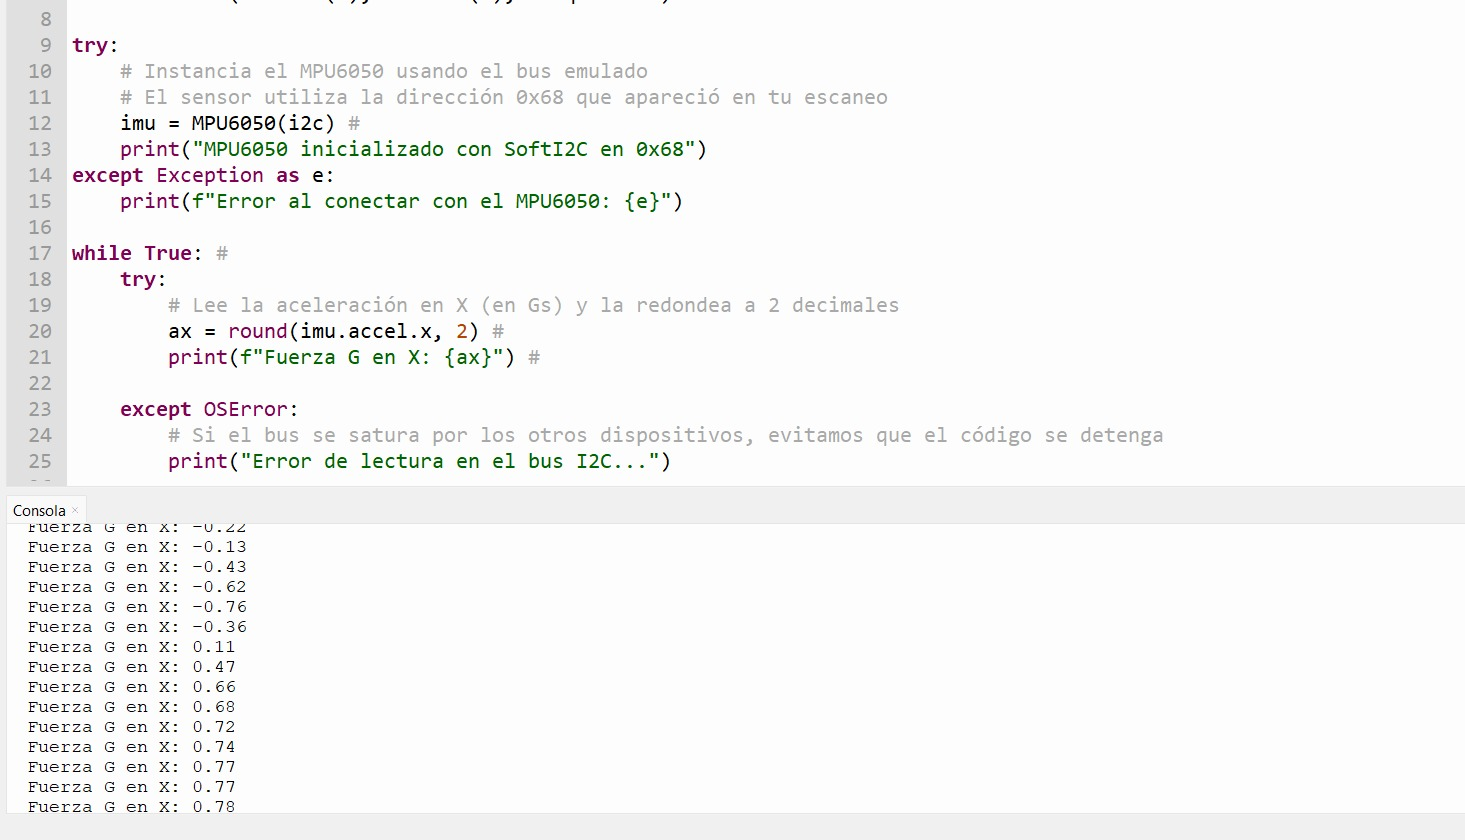
\includegraphics[width=0.85\textwidth]{img/Actividad9/Act9_1.jpg}
        \caption{Lecturas del sensor acelerómetro.}
    \end{figure}

    \subsection*{Análisis de resultados}

    Al ejecutar el programa, se observa que la Raspberry Pi Pico logra inicializar correctamente el bus I2C a 400 kHz y crear una instancia del sensor MPU6050 sin errores, lo que indica que la comunicación con el sensor es exitosa. Las lecturas del acelerómetro en el eje X ($a_x$) muestran valores cercanos a 0 g cuando el sensor está en reposo sobre una superficie plana, lo cual es coherente con la ausencia de movimiento. Al inclinar o mover la Pico, los valores de $a_x$ varían en función de la dirección y magnitud del movimiento, mostrando tanto valores positivos como negativos que reflejan la aceleración en ese eje. La capacidad de redondear a dos decimales facilita la interpretación de las lecturas, permitiendo observar cambios sutiles en la aceleración. 

    \section*{Actividad 10}

    \noindent Realizar un programa, que genere las acciones mostradas en la tabla 10-2.

        \begin{center}
        \arrayrulecolor{borderBlueA}
        \renewcommand{\arraystretch}{1.5}
        \setlength{\arrayrulewidth}{0.5pt}
        \begin{tabular}{|c|c|c|}
            \hline
            \rowcolor{headerBlueA}
            \textcolor{white}{\textbf{Condición}} & \multicolumn{2}{c|}{\textcolor{white}{\textbf{Acción}}} \\
            \hline
            \rowcolor{rowBlueA}
            $-45^\circ \leq ax \leq 45^\circ$ & LED (\textit{GPIO18}) = \textbf{\textit{OFF}} & BUZZER (\textit{GPIO17}) = \textbf{\textit{OFF}} \\
            \hline
            \rowcolor{white}
            $-46^\circ \geq ax \geq 46^\circ$ & LED (\textit{GPIO18}) = \textbf{\textit{ON}} & BUZZER (\textit{GPIO17}) = \textbf{\textit{ON}} \\
            \hline
        \end{tabular}\\[10pt]
        Tabla 10-2. Control; actividad 10
    \end{center}

    \section*{Propuesta de solución}

    Para implementar el programa que controle un LED y un buzzer en función de la aceleración medida por el sensor MPU6050, el primer paso en realizar la importación de las bibliotecas necesarias, para la conversión de radianes y grados se hace uso de la biblioteca \texttt{math}, para controlar los pines GPIO se importa la clase \texttt{Pin} y \texttt{I2C} para la comunicación con el sensor, y la clase \texttt{MPU6050} de la biblioteca \texttt{imu} para interactuar con el sensor. La últma biblioteca que se importa es \texttt{utime} para manejar los retrasos entre lecturas.

    Una vez que se definieron las bibliotecas, lo primero que se hace es configurar el bus I2C utilizando el puerto 0 de la Raspberry Pi Pico, con SDA en el pin GPIO 8 y SCL en el pin GPIO 9, a una frecuencia de 400 kHz. Luego, se crea una instancia del sensor MPU6050 pasando el objeto I2C como argumento, lo que inicializa el sensor y lo prepara para las lecturas.

    Posteriormente, se configuran los pines GPIO 17 y GPIO 18 como salidas para controlar el buzzer y el LED respectivamente.

    Por medio de un bucle infinito, se lee los valoresa de aceleración en los ejes X, Y y Z utilizando las propiedades \texttt{imu.accel.x}, \texttt{imu.accel.y} y \texttt{imu.accel.z}. Luego, se calcula el ángulo de inclinación en el eje X utilizando la función \texttt{atan2} de la biblioteca \texttt{math}, que devuelve el ángulo en radianes. Este ángulo se convierte a grados usando la función \texttt{degrees} de la misma biblioteca. Se imrpime el valor en grados para su monitoreo. Finalmente, se evalúa la condición de control: si el ángulo de inclinación en el eje X está entre -45° y 45°, se apaga el LED y el buzzer; de lo contrario, si el ángulo es menor o igual a -46° o mayor o igual a 46°, se enciende el LED y el buzzer. Se realiza un retraso de 200 milisegundos antes de la siguiente lectura utilizando \texttt{utime.sleep\_ms(200)}.

    \begin{figure}[H]
        \centering
        \begin{tikzpicture}[
            % Escalado global (puedes ajustar este parámetro)
            scale=1.0, transform shape,
            node distance=0.8cm and 0.8cm,
            every node/.style={font=\small},
            % Estilos para diagramas de flujo solicitados
            startstop/.style={rectangle, rounded corners, minimum width=3cm, minimum height=1cm, text centered, draw=black, fill=red!30},
            process/.style={rectangle, minimum width=3cm, minimum height=1cm, text centered, draw=black, fill=orange!30},
            decision/.style={diamond, aspect=2, minimum width=3cm, minimum height=1cm, text centered, draw=black, fill=green!30},
            io/.style={trapezium, trapezium left angle=70, trapezium right angle=110, minimum width=3cm, minimum height=1cm, text centered, draw=black, fill=blue!30},
            arrow/.style={thick, ->, >=stealth}
        ]
            % Nodos principales (Inicialización)
            \node (start) [startstop] {Inicio};
            \node (init) [process, below=of start, text width=6cm] {Importar librerías, inicializar I2C, IMU MPU6050 y pines (LED 18, Buzzer 17)};

            % Nodos dentro del bucle infinito
            \node (read) [process, below=of init, text width=5cm] {Leer aceleraciones\\ $a_x, a_y, a_z$};
            \node (calc) [process, below=of read, text width=5.5cm] {Calcular inclinación $X$ usando\\ trigonometría (\texttt{atan2})};
            \node (print) [io, below=of calc, text width=5cm] {Imprimir inclinación actual};

            % Nodo de decisión (Rango -45 a 45)
            \node (dec) [decision, below=of print, text width=3.5cm] {¿$-45^\circ \le X \le 45^\circ$?};

            % Ramas condicionales
            \node (off) [process, right=of dec, text width=3.5cm] {LED = OFF\\ Buzzer = OFF};
            \node (on) [process, left=of dec, text width=3.5cm] {LED = ON\\ Buzzer = ON};

            % Nodo de espera
            \node (sleep) [process, below=2cm of dec, text width=4cm] {Esperar 200 ms};

            % Conexiones lineales
            \draw [arrow] (start) -- (init);
            \draw [arrow] (init) -- (read);
            \draw [arrow] (read) -- (calc);
            \draw [arrow] (calc) -- (print);
            \draw [arrow] (print) -- (dec);

            % Conexiones de las decisiones
            \draw [arrow] (dec) -- node[above] {Sí} (off);
            \draw [arrow] (dec) -- node[above] {No (elif)} (on);

            % Convergencia hacia el final del ciclo
            \draw [arrow] (off) |- (sleep);
            \draw [arrow] (on) |- (sleep);

            % Retorno del bucle infinito (while True)
            % Sale del sur del nodo sleep, baja un poco, rodea el nodo "on" por la izquierda y sube al nodo "read"
            \draw [arrow] (sleep.south) -- ++(0,-0.5) -| ([xshift=-1.5cm]on.west) |- (read.west);

        \end{tikzpicture}
    \end{figure}

    \section*{Desarrollo}

    \lstinputlisting[language={[LAB]Python}, caption=Código de la Actividad 10, basicstyle=\ttfamily\scriptsize]{Code/Act10.py}

    \begin{figure}[H]
        \centering
        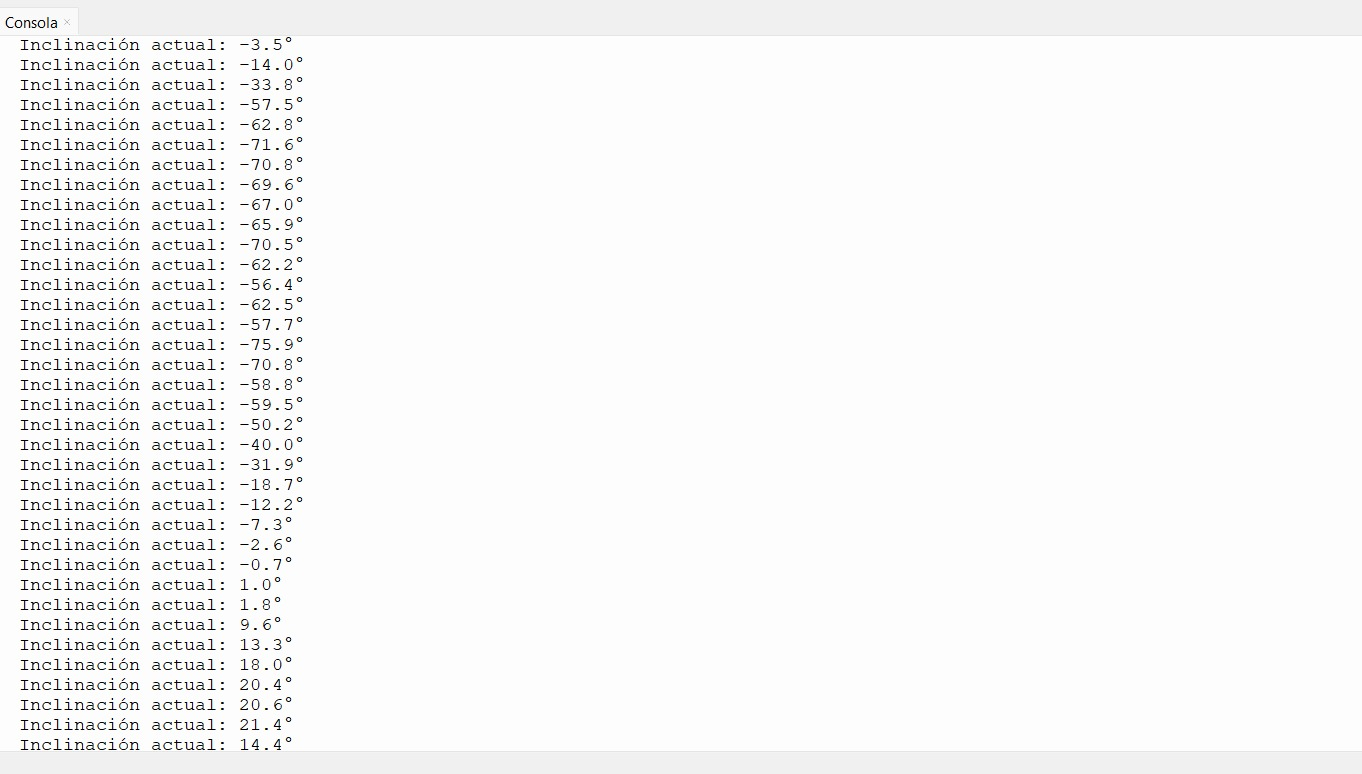
\includegraphics[width=0.85\textwidth]{img/Actividad10/Act10_3.jpg}
        \caption{Lecturas del sensor acelerómetro - Actividad 10.}
    \end{figure}


    \begin{figure}[H]
        \centering
        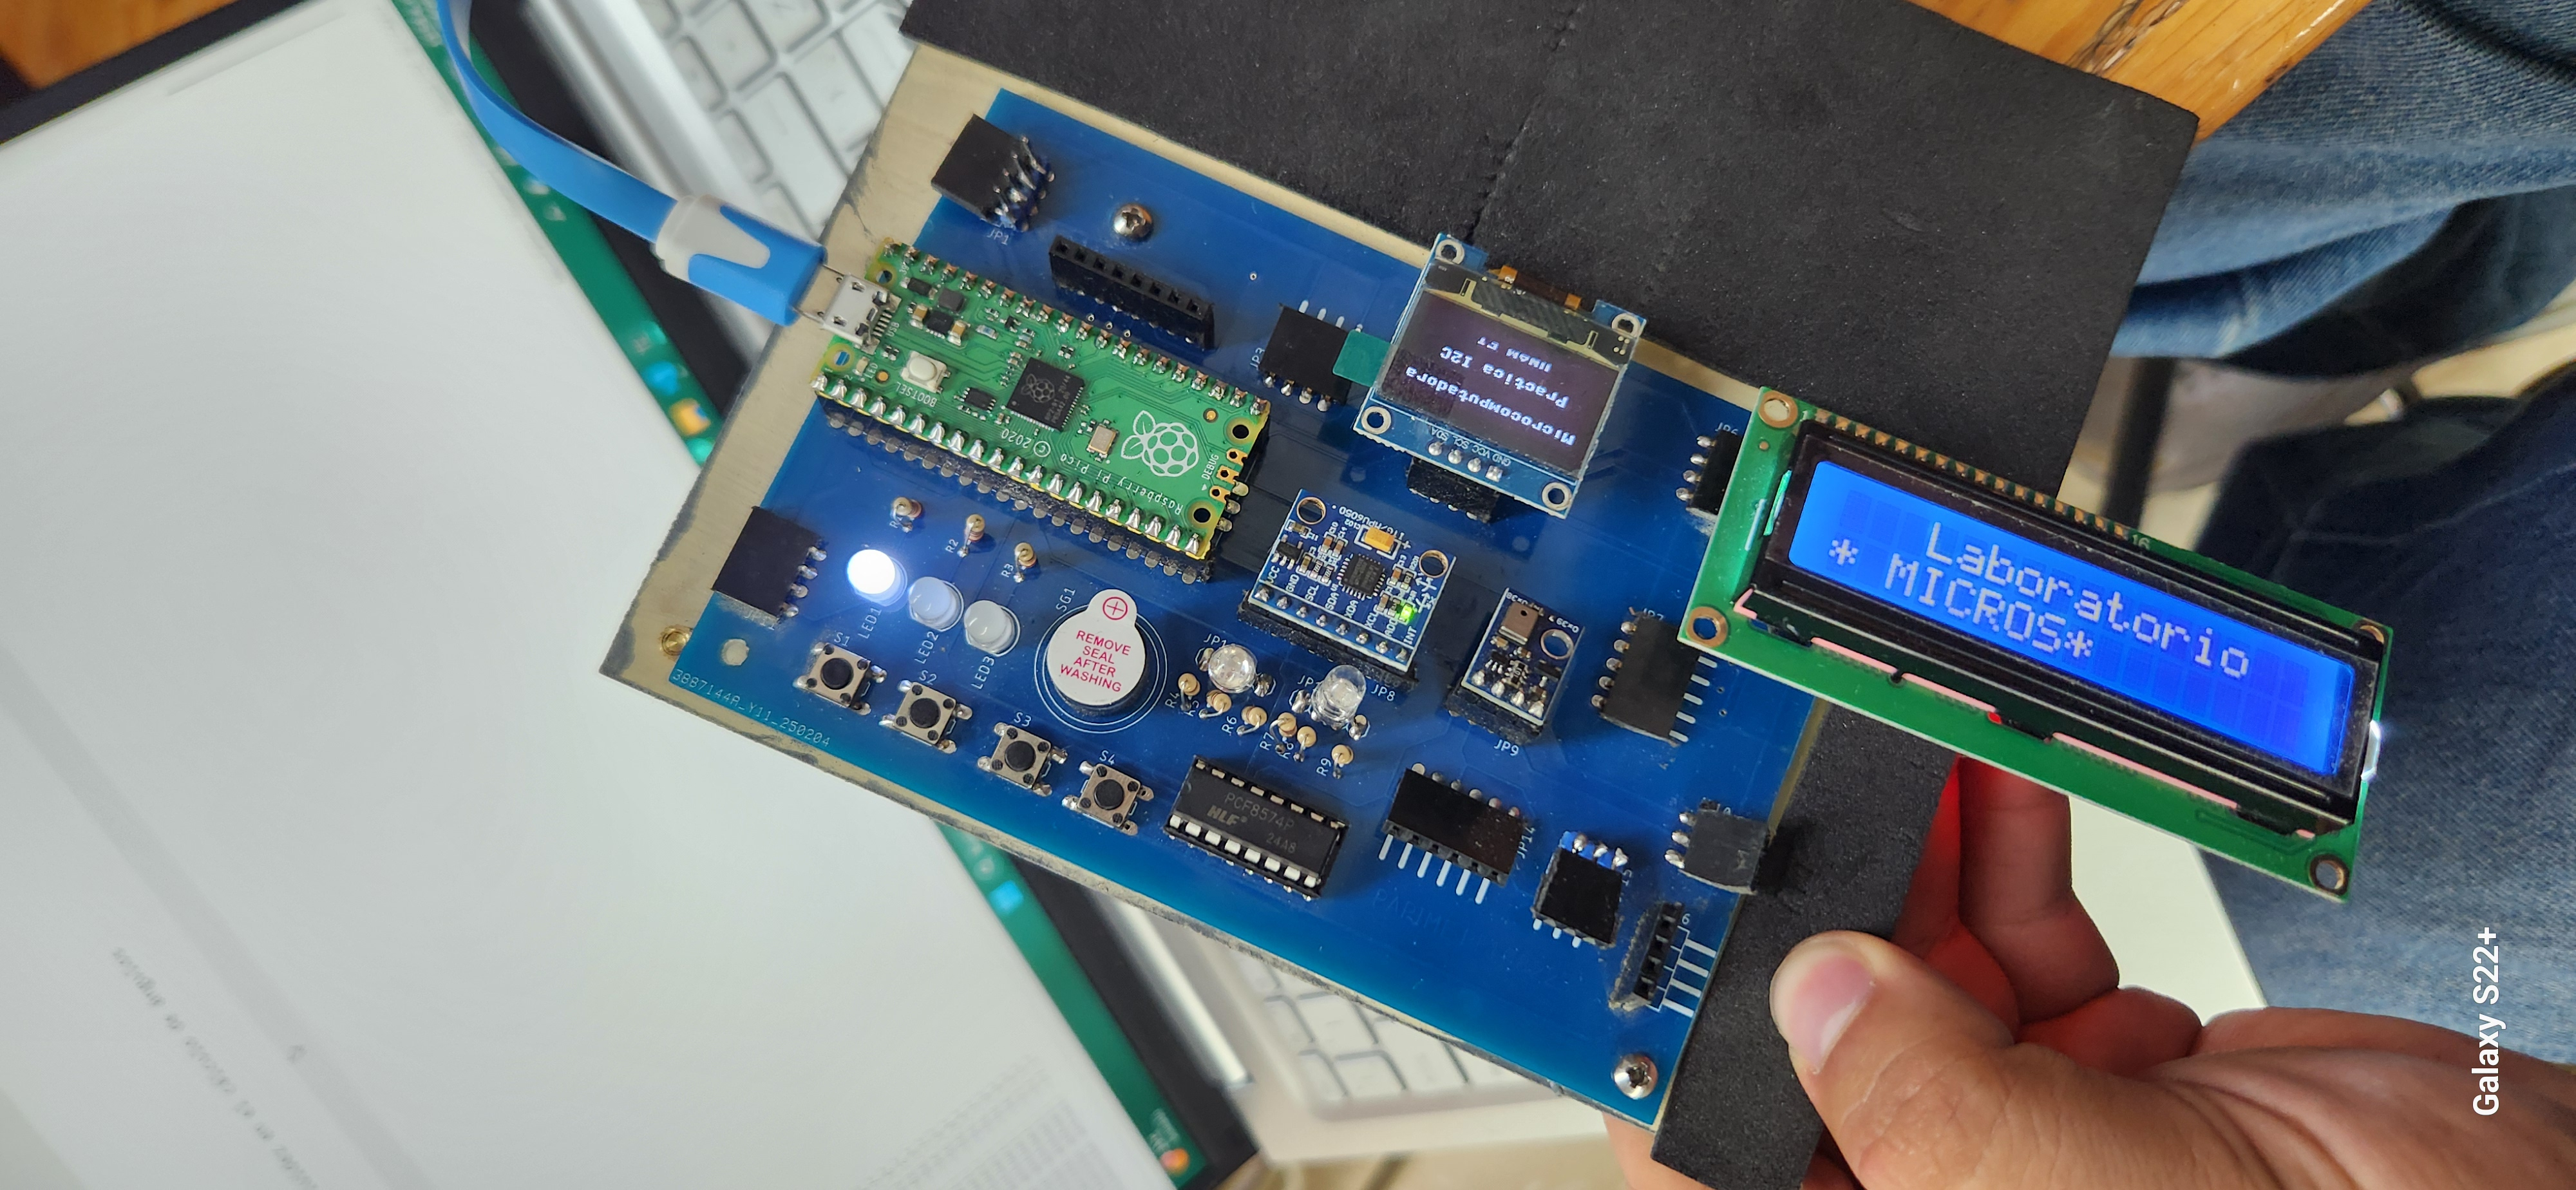
\includegraphics[width=0.85\textwidth]{img/Actividad10/Act10_1.jpg}
        \caption{Inclinación del sensor acelerómetro mayor a 46$^\circ$ y menor a -46$^\circ$ - Actividad 10.}
    \end{figure}

    \begin{figure}[H]
        \centering
        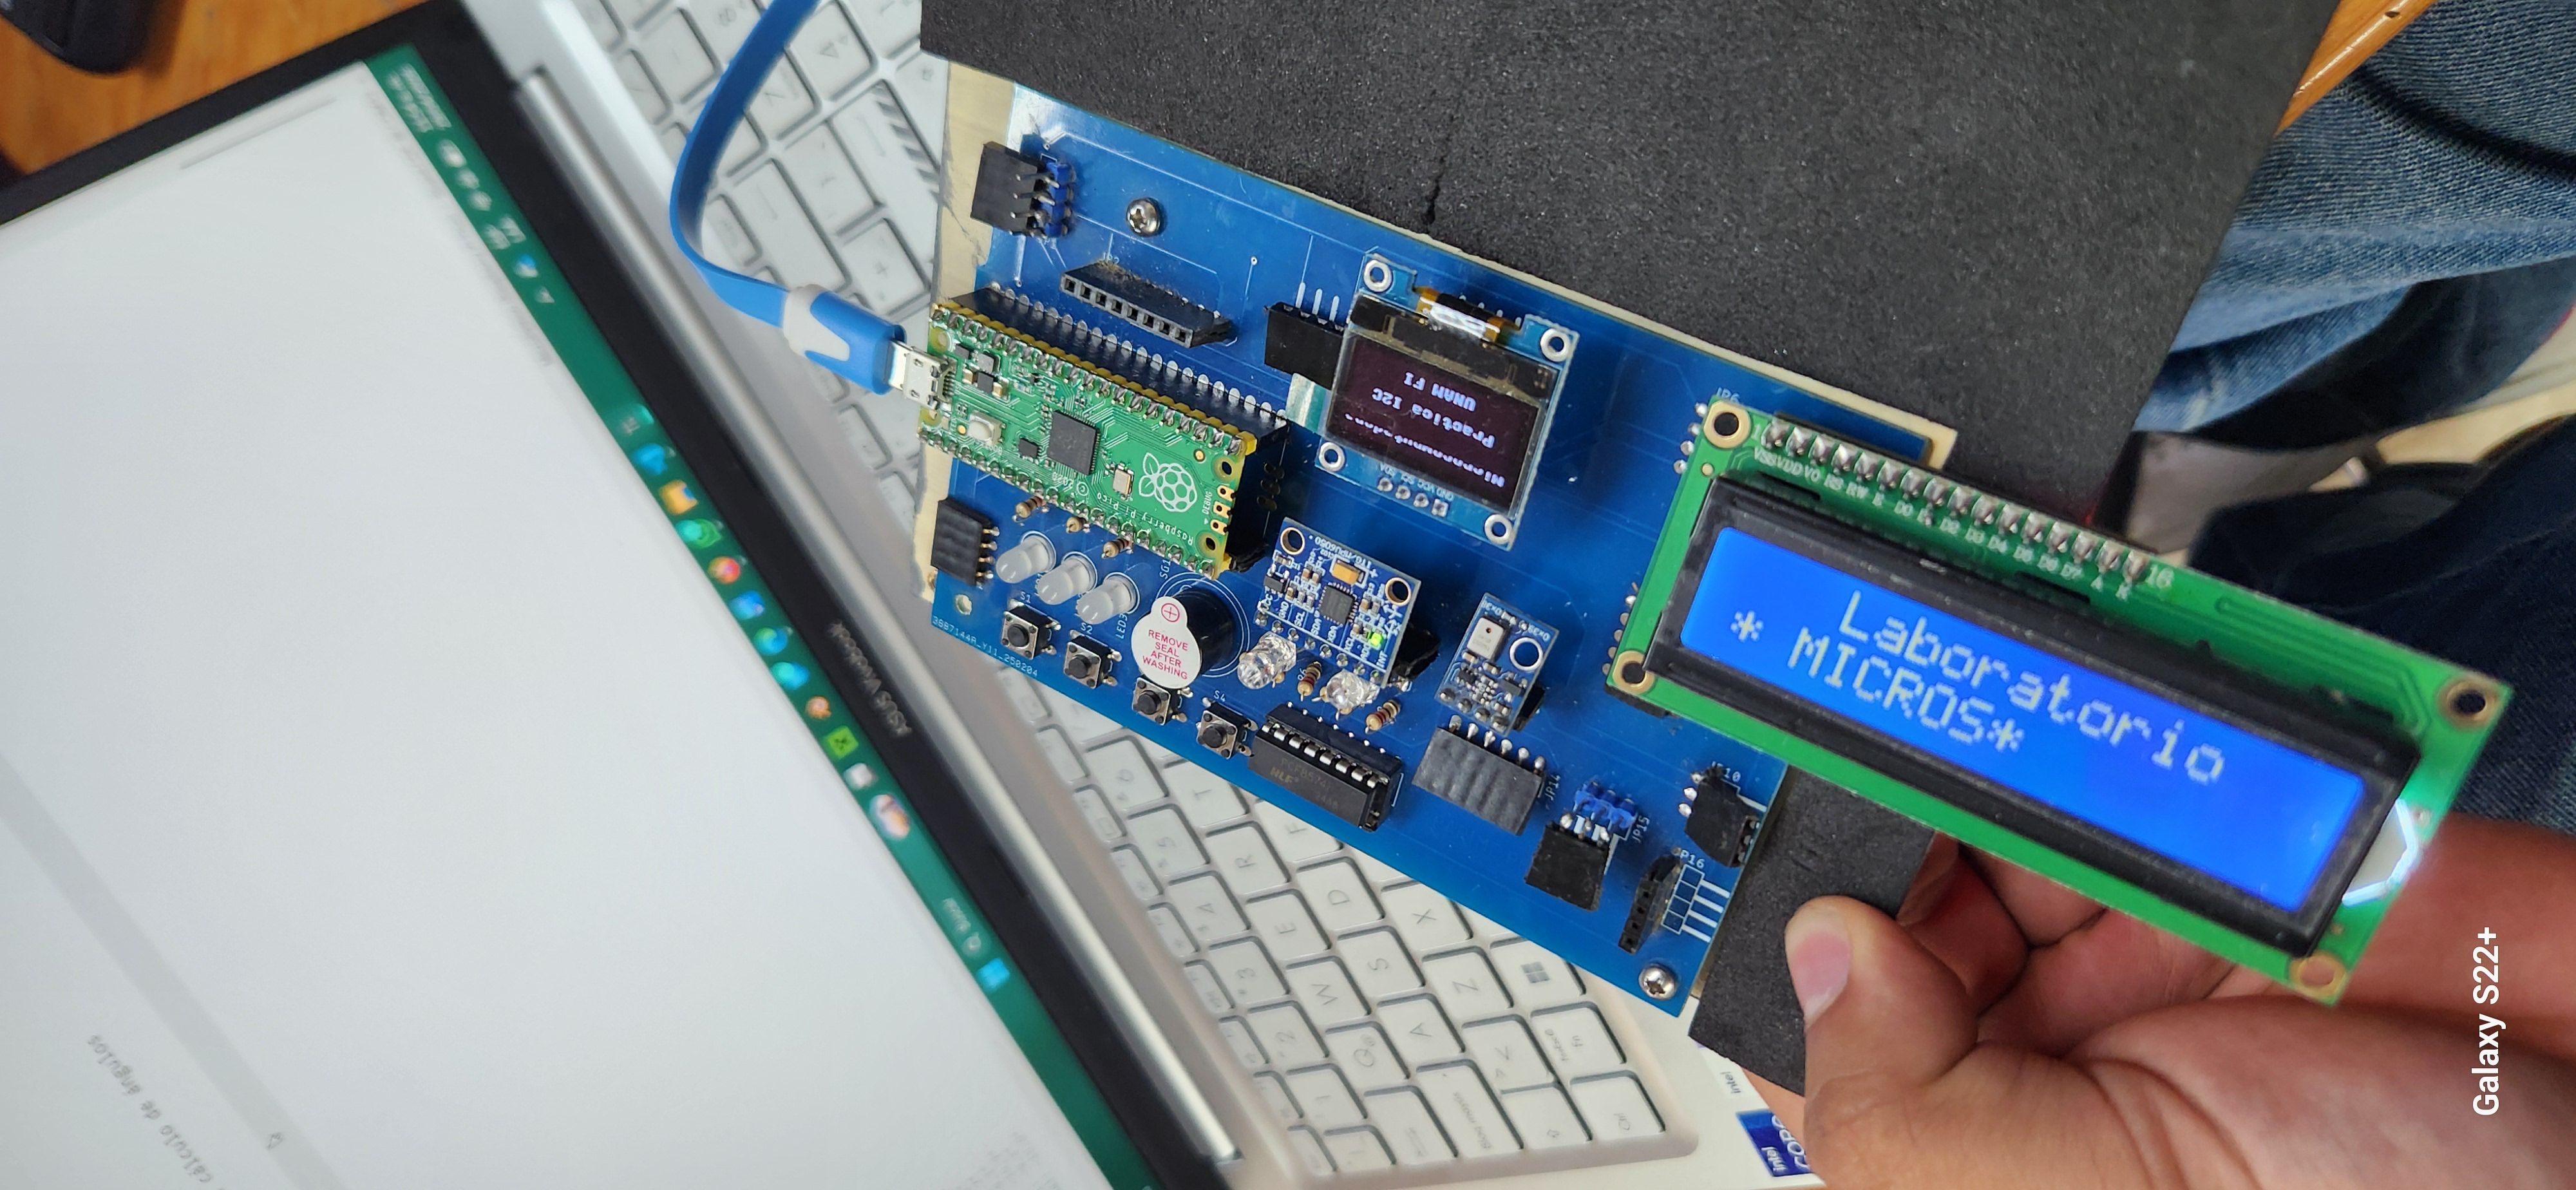
\includegraphics[width=0.85\textwidth]{img/Actividad10/Act10_2.jpg}
        \caption{Inclinación del sensor acelerómetro entre -45$^\circ$ y 45$^\circ$ - Actividad 10.}
    \end{figure}

    \subsection*{Análisis de resultados}

    Al ejecutar el programa, se observa que la Raspberry Pi Pico logra inicializar correctamente el bus I2C a 400 kHz, crear una instancia del sensor MPU6050 y configurar los pines para el LED y el buzzer sin errores, lo que indica que la comunicación con el sensor y la configuración de los GPIO es exitosa. Las lecturas del acelerómetro permiten calcular la inclinación en el eje X, mostrando valores en grados que varían según la posición del sensor. Cuando la inclinación supera los 46° o es menor a -46°, el LED se enciende y el buzzer suena, indicando que se ha detectado una inclinación fuera del rango permitido. Por otro lado, cuando la inclinación está entre -45° y 45°, el LED permanece apagado y el buzzer está silenciado, lo que confirma que el sistema de control responde correctamente a las condiciones establecidas. El retraso de 200 ms entre lecturas permite un monitoreo continuo sin saturar la consola con demasiada información.


    \newpage
    \section{Conclusiones:}

    \begin{itemize}
        \item \textbf{Espinoza Matamoros Percival Ulises:} 
        
        Por medio de la realización de esta práctica, he logrado comprender a fondo el funcionamiento del protocolo de comunicación I2C y su integración con la Raspberry Pi Pico. Ya que a travez del protocolo de comunicación se pueden conectar múltiples dispositivos utilizando solo dos líneas de comunicación (SDA y SCL), lo que simplifica el diseño del hardware y permite una mayor flexibilidad en la conexión de periféricos. La función \texttt{scan()} fue esencial para identificar las direcciones hexadecimales de los dispositivos conectados al bus, lo que facilitó la configuración y uso de componentes como el expansor PCF8574, el display OLED SSD1306 y el sensor TMP102. 

        Trabajar con diferentes dispositivos me permitió apreciar la versatilidad del protocolo I2C, ya que cada componente mantiene su propia dirección hexadecimal para ser identificado dentro del bus por el bus master de la Pico. De igual forma es importante destacar que el usar MicroPython en la Raspberry Pi Pico hizo que el proceso de desarrollo fuera más sencillo y accesible, permitiendo una rápida implementación y prueba de los diferentes periféricos conectados al bus I2C, ya que para instanciar los objetos correspondientes a los sensores, en la mayoría de los casos, solo se requiere pasar el objeto I2C como argumento, lo que simplifica la interacción con los dispositivos y acelera el proceso de desarrollo.

        \item \textbf{Flores Colin Victor Jaziel:} 
        
        En esta practica número 10 he comprendido el funcionamiento y la versatilidad del protocolo de comunicacion I2C en combinación con el manejo de la Raspberry Pi Pico. A traves del desarrollo de las diferentes actividades, comprobe como un bus de comunicacion de solo dos lineas (SDA y SCL) permite conectar y controlar multiples perifericos simultaneamente, simplificando drasticamente el diseno del hardware. La funcion \texttt{scan()} resulto fundamental en cada actividad para identificar las direcciones hexadecimales de los dispositivos conectados al bus, confirmando la presencia del expansor PCF8574 (0x39), del display OLED SSD1306 (0x3C) y del sensor TMP102 (0x48) antes de proceder con su configuracion y uso.

        Al trabajar con distintos dispositivos como el expansor de entradas y salidas PCF8574 (actividad 2), la pantalla OLED SSD1306 (actividad 6), y el sensor de temperatura TMP102 (actividad 7), pude poner a prueba la flexibilidad de este protocolo. Observar como cada componente mantiene su propia direccion hexadecimal para ser identificado dentro del bus por el bus master de la Pico, me dejo muchisimo mas claro el flujo de este protocolo maestro-esclavo en aplicaciones del mundo real.

        \item \textbf{Lara Hernandez Angel Husiel:} 
        
        En esta práctica el funcionamiento y la versatilidad del protocolo de comunicación I2C integrado con la Raspberry Pi Pico. A través del desarrollo de las diferentes actividades, comprendí cómo un bus de comunicación de solo dos líneas (SDA y SCL) permite conectar y controlar múltiples periféricos simultáneamente, simplificando drásticamente el diseño del hardware y liberando pines GPIO.

        Al trabajar con distintos dispositivos como el expansor de entradas y salidas PCF8574, la pantalla LCD I2C, y sensores complejos como el TMP102, el AHT10 (de temperatura y humedad) y el MPU6050 (acelerómetro y giroscopio), pude poner a prueba la flexibilidad de este protocolo. Observar cómo cada componente mantiene su propia dirección hexadecimal para ser identificado dentro del bus por el bus master de la Pico, me dejó muchísimo más claro el flujo de este protocolo maestro-esclavo en aplicaciones del mundo real.
        
    \end{itemize}

    \newpage


    \nocite{*} 
    \printbibliography[heading=bibintoc, title={Referencias}]

\end{document}